\documentclass[3p,11pt,authoryear]{elsarticle}  %preprint, 1p/3p/5p journal
\usepackage{setspace}
\onehalfspacing

\input{setup.tex}
\journal{Transportation Research Part E: Logistics and Transportation Review}


%%%%%%%%%%%%%%%%
\begin{document}
%%%%%%%%%%%%%%%%

\begin{frontmatter}


\title{Scheduling long-haul battery-electric trucks: coordinating charging, breaks, and daily rests}
%\title{Scheduling long-haul battery-electric trucks: coordinating charging and driver regulations}
%
%\title{The multi-day electric vehicle truck driver scheduling problem: Coordinating charging, breaks, and daily rests}

%Synchronizing charging and driver regulations in long-haul battery-electric freight transport

%The multi-day electric vehicle truck driver scheduling problem

\author[indokaddress]{Steffen J.S. Bakker\corref{cor}} 
            \ead{steffen.bakker@ntnu.no}
            \author[indokaddress]{Mostafa Mohammadi}
            \author[indokaddress]{Johan Stafseng}
            \author[indokaddress]{Magnus Stålhane}
            \author[sintefaddress]{Odd André Hjelkrem}

		\cortext[cor]{Corresponding author}
		\address[indokaddress]{Department of Industrial Economics and Technology Management, Norwegian University of Science and Technology, Alfred Getz veg 3, NO-7491 Trondheim, Norway}
        \address[sintefaddress]{Department of Energy Systems, SINTEF Energy Research - Trondheim, Norway}


\begin{abstract}
Recent advances in battery technology and fast charging are making long-haul battery-electric freight transport increasingly feasible. As vehicle ranges extend beyond regional distribution, charging decisions become increasingly intertwined with Hours-of-Service regulations. Since charging is time-consuming and unavoidable on long routes, operators must ensure that vehicles remain sufficiently charged while complying with driver regulations. Efficient operation therefore depends on synchronizing charging activities with mandatory driver breaks and daily rest periods.
%
We study this scheduling problem for battery-electric trucks operating on multi-day long-haul routes. We introduce a multi-day electric truck driver scheduling problem in which charging decisions are optimized jointly with Hours-of-Service compliance to minimize total route duration. 
The problem is formulated as a resource-constrained shortest path problem and solved using an exact labeling algorithm that jointly models battery dynamics and driver regulations.
Computational experiments show that optimized battery-electric truck schedules can, under favorable charging conditions, be completed within \red{XX\%} of the duration of equivalent diesel-truck operations. However, schedule feasibility and performance deteriorate rapidly when charging opportunities are sparse or charging power is insufficient. 
Compared with a simpler charging strategy, the proposed optimization approach reduces route durations by up to \red{XX\%}. Moreover, allowing partial recharging provides modest but consistent reductions in route time relative to full recharging. The results demonstrate that synchronization of charging and mandatory driver interruptions is a key operational enabler of long-haul freight electrification.
\end{abstract}



% Fill in data. If unknown, outcomment the field
\begin{keyword}
Battery-electric trucks; long-haul freight transport; hours-of-Service regulations; charging scheduling; driver scheduling; resource-constrained shortest path.
\end{keyword}
%\HISTORY{Received: Month DD, YYYY; Accepted: Month DD, YYYY; Published Online: Month DD, YYYY}

\end{frontmatter}

%%%%%%%%%%%%%%%%%%%%%%%%%%%%%%%%%%%%%%%%%%%%%%%%%%%%%%%%%%%%%%%%%%%%%%


\section{Introduction}
\label{sec:Intro}


% Motivation
The electrification of road freight transport has progressed rapidly over the last decade. Battery-electric trucks are now being adopted in urban distribution and regional logistics, where vehicles can typically recharge at depots or terminals during predictable off-duty periods \citep{shoman2023battery}. Recent improvements in battery capacity and fast-charging technology are extending feasible driving ranges and making battery-electric trucks increasingly viable for long-haul freight operations. Current commercial vehicle offerings illustrate this development: heavy-duty battery-electric trucks are commonly marketed with single-charge ranges of around 300 km, while newer long-haul models target approximately 500 km under favorable operating conditions \citep{volvofhElectric,mercedesEactros600}. However, road freight transport is a highly competitive business with low profit margins \citep{eu2025roadcharges}, where schedules are tight and time losses translate directly into cost. If charging causes additional time losses,  battery-electric trucks can quickly become unattractive for long-haul freight operations.

% Operational challenge + Synchronization of charging and Hours-of-Service requirements
A defining feature of long-haul trucking is that operations are constrained by Hours-of-Service (HoS) regulations. Under EU regulation, drivers must take mandatory breaks and daily rest periods, typically taken overnight, that reset driving and working-time limits \citep{goel2017exact}. Traditionally, compliance with these regulations has been the primary scheduling challenge, as diesel refueling is fast and widely available. Consequently, refueling is rarely modeled as a binding scheduling resource in conventional truck operations \citep{schulz2024ipc}. For battery-electric trucks, in contrast, charging is substantially more time-consuming than diesel refueling and depends on the availability of suitable charging infrastructure. Operators must therefore ensure that vehicles remain sufficiently charged while simultaneously complying with driver regulations. 
Efficient operation depends on synchronizing charging activities with mandatory breaks and daily rests such that charging can be absorbed into periods during which the driver is already required to be off duty. 
%The extent to which charging can be effectively synchronized with mandatory driver interruptions, and how this affects route duration, schedule feasibility, and the competitiveness of long-haul battery-electric trucking, remain largely unexplored.

In this paper, we investigate the synchronization of charging activities with mandatory breaks and daily rests in long-haul battery-electric freight transport. We study a multi-day scheduling problem in which charging, breaks, and daily rests must be jointly planned to minimize route duration while satisfying both Hours-of-Service and energy constraints.

\subsection{Related literature}

% Related literature: Truck driver scheduling under Hours-of-Service regulations
The Truck Driver Scheduling Problem (TDSP) concerns the construction of driver schedules that satisfy regulatory HoS constraints while optimizing operational objectives such as route duration or transportation cost. The Truck Driver Scheduling Problem (TDSP) has been studied extensively under Hours-of-Service regulations \citep{archetti2009trip, goel2012minimum, goel2012truck}. %both EU and USA

Methodologically, TDSPs are commonly formulated as shortest path problems with resource constraints (SPPRCs). Feasible schedules are constructed incrementally through labeling algorithms that extend partial paths while tracking resources such as accumulated driving and working time since the last break or rest. Resource extension functions are used to update resource states and identify infeasible path extensions \citep{goel2010truck, drexl2010labelling}. Building on this paradigm, \citet{goel2017exact} introduced an exact branch-and-price framework with a parameter-free network representation that avoids time discretization, while preserving regulatory feasibility. However, these models assume conventional vehicles with negligible refueling times and do not consider energy constraints.


% Related literature: Electric vehicle routing and charging
While TDSP research focuses on regulatory feasibility, the Electric Vehicle Routing Problem (EVRP) literature provides a rich body of work on modeling battery dynamics and charging decisions \citep{schneider2014electric, han2025uncertainty}. 
%Charging is time-consuming and depends on the availability of suitable charging infrastructure. 
%and may be performed partially or fully. 
Many exact EVRP approaches are based on branch-and-price frameworks in which a master problem selects vehicle routes, while SPPRC pricing problems generate new feasible routes. In these formulations, battery state is treated as a resource and charging duration directly affect route timing \citep{desaulniers2016exact, lam2022branch, nafstad2025branch}. Several works allow partial recharging and nonlinear charging functions to better reflect operational practice \citep{montoya2017electric, froger2019improved}. Whereas most EVRP studies focus on route construction and charging decisions along a route, recent work has begun to integrate routing decisions with the scheduling of charging infrastructure. For example, \citet{yamin2025electric} jointly optimize urban delivery routes and overnight depot-charging schedules using a branch-price-and-cut algorithm. Their formulation accounts for nonlinear charging and limited charging capacity, but does not consider HoS-constrained driver schedules.
%kicked out: \citep{bruglieri2023matheuristic}


%interaction charging and HoS scheduling -> gap
Only a limited number of studies explicitly consider the interaction between charging activities and driver breaks and rests under HoS regulation. \citet{schiffer2017impact} extend the EVRP by incorporating HoS regulations and allowing en-route charging activities to be synchronized with mandatory driver breaks. Their EVRP is motivated by one-day routing and scheduling of electric commercial delivery vehicles in regional distribution networks. They solve the problem using a mixed-integer formulation combined with an adaptive large neighborhood search heuristic.
Closer to the long-haul setting considered in this paper, \citet{wan2024longhaul} study an opportunity-charging planning problem for a battery-electric truck in a single freight corridor case study. Their model coordinates charging decisions with planned stops at highway service areas and logistics hubs while accounting for charging technologies, electricity prices, and temporal flexibility. However, HoS regulations are represented only through simplified driving-time and rest constraints and the model does not consider recurring daily-rest requirements.
More recently, \citet{brockmann2025breakandcharge} develop a mathematical programming model for an Electric Vehicle Truck Driver Scheduling Problem (EVTDSP) in which charging operations and mandatory driver breaks are jointly optimized. %, and evaluate it using real-world data from Northwest Germany. 
Their analysis highlights the importance of accounting for driver regulations when assessing the operational performance of battery-electric trucks. However, the study is restricted to single-day operations and does not consider recurring daily rests or multi-day scheduling decisions.
Finally, \citet{schneider2023novel} analyze one-day electric truck operations and evaluate predefined charging and EU HoS-complient break strategies, including alternatives enabled by high-power charging technologies such as the Megawatt Charging System. While their study provides valuable insights into the interaction between charging technology and driver regulations, it only evaluates a limited number of predefined operating strategies and does not address the underlying scheduling problem.




\subsection{Research gap and contributions}

%GAP
It remains unclear to what extent charging can be absorbed within mandatory driver breaks and daily rests in multi-day long-haul operations, and how incomplete synchronization affects route duration and schedule feasibility. Existing studies focus primarily on distribution networks and single-day operations, whereas multi-day operations involve repeated charging, mandatory breaks, and recurring daily rests, creating greater potential for both synergies and conflicts between energy and regulatory requirements. Furthermore, existing synchronization studies rely primarily on mixed-integer formulations and heuristic solution approaches and do not provide an exact method for jointly optimizing charging, breaks, and daily rests over multiple days.

% Contributions
To address this gap, we study a multi-day variant of the Electric Vehicle Truck Driver Scheduling Problem (EVTDSP), which determines how charging activities, mandatory breaks, and daily rest periods should be scheduled and synchronized in long-haul battery-electric freight operations. Given a prescribed route and a set of charging opportunities, the objective is to minimize total route duration while satisfying both HoS and battery constraints.

The contributions of this paper are threefold. First, we extend the truck driver scheduling problem to the multi-day battery-electric setting by explicitly integrating charging decisions with both mandatory breaks and recurring daily rest periods. Second, we develop an exact resource-constrained shortest path formulation and labeling algorithm by extending the framework of \citet{goel2017exact} with battery dynamics, tailored resource extension functions, and dominance rules. %The resulting method jointly enforces HoS and energy feasibility without time discretization.
Third, we introduce an open-source benchmark set for the EVTDSP informed by interviews and operational data collected from long-distance trucking companies in Norway and Northern Europe, and use it to systematically analyze how route structure, charging conditions, and rest requirements affect schedule feasibility, charging-rest synchronization, and the value of partial recharging.



% Research objectives (alreadu in contributions!!)
%Beyond the development of an exact optimization framework, this paper seeks to understand how charging requirements interact with Hours-of-Service regulations in long-haul battery-electric truck operations. In particular, we examine how route structure, charging infrastructure, and charging strategies affect route duration and schedule feasibility.


\begin{comment}
    \begin{table}
\TABLE
{Comparative overview of related works.\label{tab:Literature_Review}}
{\begin{tabular}{@{}p{7.5cm}p{2.2cm}p{3cm}ccccc@{}}
\hline\up
\textbf{Paper} & \textbf{Objective Function} & \textbf{Solution Method} & \textbf{TDS} & \textbf{CS} & \textbf{LCF} & \textbf{MS} & \textbf{LH} \\
\hline\up
\cite{xue2025routing} & Min Time & DP & Yes & Yes & Yes & Yes & Yes \\
\cite{archetti2009trip} & None & PA & Yes & No & No & Yes & No \\
\cite{barco2017optimal} & Min Cost & DEA & No & Yes & No & No & No \\
\cite{campbell2004efficient} & MCO & Heuristic & Yes & No & No & Yes & No \\
\cite{ceselli2009column} & Min Cost & CG, DP & Yes & No & No & No & No \\
\cite{conrad2011recharging} & MCO & Heuristics & No & No & Yes & No & No \\
\cite{de2022using} & Min Cost & DP, Heuristics & No & No & Yes & Yes & Yes \\
\cite{desaulniers2016exact} & Min Cost & BNPNC & No & Yes & Yes & No & No \\
\cite{drexl2010labelling} & MCO & DP & Yes & No & No & Yes & Yes \\
\cite{dolgui2024scheduling} & Min Distance & Heuristics & No & Yes & No & No & Yes \\
\cite{ferro2020optimal} & Min Cost & MIP & No & Yes & Yes & No & No \\
\cite{froger2019improved} & Min Time & DP, Heuristic & No & Yes & No & No & No \\
\cite{goel2009vehicle} & MCO & Heuristic, LNS & Yes & No & No & Yes & No \\
\cite{goel2010truck} & None & BFS & Yes & No & Yes & Yes & Yes \\
\cite{goel2012canadian} & Min Time & DP & Yes & No & Yes & Yes & Yes \\
\cite{goel2012minimum} & Min Time & DP & Yes & No & Yes & Yes & Yes \\
\cite{goel2017exact} & Min Cost & DP & Yes & No & Yes & Yes & Yes \\
\cite{goel2012efficient} & None & DFBSS & Yes & No & No & Yes & Yes \\
\cite{vidal2020concise} & Min Cost & HGSADC & Yes & Yes & No & Yes & Yes \\
\cite{grandinetti2016pick} & MCO & MIP, WSM & No & Yes & Yes & No & No \\
\cite{keskin2019electric} & MCO & Matheuristic & No & No & No & Yes & No \\
\cite{kocc2018long} & Min Cost & Matheuristics, ALNS & Yes & No & No & Yes & Yes \\
\cite{kok2010dynamic} & MCO & DP, Heuristic & Yes & No & No & Yes & Yes \\
\cite{lam2022branch} & Min Cost & BNCNP & No & Yes & No & No & No \\
\cite{lin2016electric} & Min Cost & MIP & No & Yes & Yes & No & No \\
\cite{mayerle2020long} & Min Cost & LNS & Yes & No & No & Yes & Yes \\
\cite{montoya2017electric} & Min Time & Hybrid Metaheuristic & No & Yes & No & No & No \\
\cite{pelletier2018charge} & Min Cost & MIP & No & No & No & Yes & No \\
\cite{prescott2010european} & Min Cost & LNS, labeling & Yes & No & No & Yes & No \\
\cite{rancourt2013long} & MCO & Tabu Search & Yes & No & No & Yes & Yes \\
\cite{savelsbergh1998drive} & MCO & BNP & Yes & No & No & Yes & No \\
\cite{schiffer2017impact} & Min Cost & MIP, ALNS & Yes & Yes & Yes & No & No \\
\cite{schneider2014electric} & MCO & Hybrid Heuristic & No & Yes & Yes & No & Yes \\
\cite{schneider2023novel} & None & -- & Yes & Yes & No & Yes & Yes \\
\cite{tilk2020bidirectional} & Min Cost & BNCNP, DP & Yes & No & No & Yes & Yes \\
\cite{vital2021scheduling} & Min Cost & DP & Yes & No & Yes & No & No \\
\cite{xu2003solving} & Min Cost & Matheuristics, DP & Yes & No & Yes & No & No \\
Current Study & Min Cost & DP & Yes & Yes & Yes & Yes & Yes \down\\
\hline
\end{tabular}}
{TDS = Truck Driver Scheduling, CS = Charging Stations, LCF = Linear Charging Function, MS = Multiple Shifts, LH = Long-Haul.}
\end{table}
% 
\end{comment}



    %------------------------------------------------%
    
    \section{Problem definition}
    
    %------------------------------------------------%
    
    
This paper studies the Electric Vehicle Truck Driver Scheduling Problem (EVTDSP), which concerns the construction of HoS-compliant and energy-feasible schedules for a battery-electric truck operating on a long-haul route. Given a predefined sequence of customer visits, the objective is to minimize the total route duration by determining the timing of mandatory breaks and daily rests, as well as the timing, location, and amount of battery charging. Figure~\ref{fig:evtdsp_route} illustrates the route structure considered in the problem: the truck travels from origin $o$ to destination $d$ through a predetermined sequence of $N$customers, with charging stations available along the route.
\begin{figure}[htbp!]
\centering

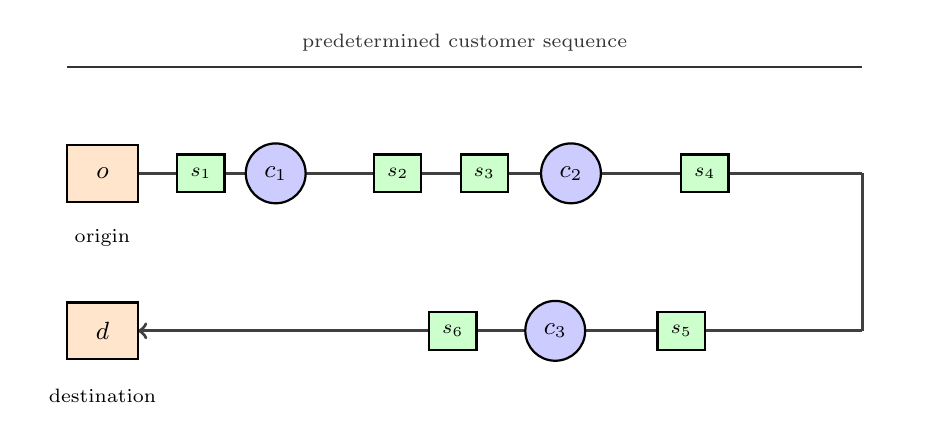
\begin{tikzpicture}[x=1cm,y=1cm]

% Fixed bounding box keeps the whole diagram geometrically centered
\path[use as bounding box] (-0.25,-2.95) rectangle (10.85,1.85);

% ===================== guide line =====================
% Aligned with the full horizontal extent of the route
\draw[thin,color=black!80]
    (0.25,1.35) --
    node[midway,above=2pt]
    {\scriptsize predetermined customer sequence}
    (10.35,1.35);

% ===================== route =====================
% Upper route
\draw[very thick,color=black!75]
    (1.15,0) -- (10.35,0);

% Downward turn
\draw[very thick,color=black!75]
    (10.35,0) -- (10.35,-2.0);

% Lower route, ending at destination
\draw[very thick,->,color=black!75]
    (10.35,-2.0) -- (1.15,-2.0);

% ===================== origin =====================
\draw[thick,fill=orange!20]
    (0.25,-0.36) rectangle (1.15,0.36);
\node at (0.70,0) {\small $o$};
\node at (0.70,-0.82) {\scriptsize origin};

% ===================== destination =====================
\draw[thick,fill=orange!20]
    (0.25,-2.36) rectangle (1.15,-1.64);
\node at (0.70,-2.0) {\small $d$};
\node at (0.70,-2.82) {\scriptsize destination};

% ===================== upper-row customers =====================
\draw[thick,fill=blue!20] (2.90,0) circle (0.38);
\node at (2.90,0) {\small $c_1$};

\draw[thick,fill=blue!20] (6.65,0) circle (0.38);
\node at (6.65,0) {\small $c_2$};

% ===================== upper-row charging stations =====================
\draw[thick,fill=green!20]
    (1.65,-0.24) rectangle (2.25,0.24);
\node at (1.95,0) {\scriptsize $s_1$};

\draw[thick,fill=green!20]
    (4.15,-0.24) rectangle (4.75,0.24);
\node at (4.45,0) {\scriptsize $s_2$};

\draw[thick,fill=green!20]
    (5.25,-0.24) rectangle (5.85,0.24);
\node at (5.55,0) {\scriptsize $s_3$};

\draw[thick,fill=green!20]
    (8.05,-0.24) rectangle (8.65,0.24);
\node at (8.35,0) {\scriptsize $s_4$};

% ===================== lower-row customer =====================
\draw[thick,fill=blue!20] (6.45,-2.0) circle (0.38);
\node at (6.45,-2.0) {\small $c_3$};

% ===================== lower-row charging stations =====================
% Travel direction on the lower row is from right to left:
% s5 -> c3 -> s6 -> d
\draw[thick,fill=green!20]
    (7.75,-2.24) rectangle (8.35,-1.76);
\node at (8.05,-2.0) {\scriptsize $s_5$};

\draw[thick,fill=green!20]
    (4.85,-2.24) rectangle (5.45,-1.76);
\node at (5.15,-2.0) {\scriptsize $s_6$};

\end{tikzpicture}

\caption{Illustrative route structure for the EVTDSP. The truck travels
from origin $o$ to destination $d$ through a predetermined sequence of
customers $(c_1,c_2,c_3)$, with charging stations $(s_1,\ldots,s_6)$
available along the route.}
\label{fig:evtdsp_route}
\end{figure}
Let the predetermined route be represented by the ordered sequence of mandatory locations $\mathcal{R}=(c_0,c_1,\ldots,c_N,c_{N+1})$, where $c_0$ denotes the origin, $c_{N+1}$ the destination, and the intermediate locations correspond to customer visits. Consecutive locations $(c_i,c_{i+1})$ define route legs. Moreover, let $\mathcal{L}$ denote the set of all route \emph{legs}, i.e., $\mathcal{L}=\left\{(c_i,c_{i+1}) \mid i=0,\ldots,N-1\right\}$. Charging stations may be located along a leg. Let $\mathcal{P}$ denote the ordered set of physical nodes obtained by inserting all charging stations into the route. Consequently, each {leg} may be decomposed into one or more \emph{sublegs} connecting consecutive physical nodes in $\mathcal{P}$.
\red{introduce a short table with notation? There are some things in the paper not defined.}

Service at each customer requires a fixed, non-interruptible duration. Distances and travel times between consecutive physical locations are assumed known. % and deterministic. 
Energy consumption is proportional to distance traveled and independent of cargo load. The vehicle is equipped with a battery of fixed capacity %, measured in kwH 
and may recharge at charging stations located along the route. Charging stations are assumed homogeneous and provide energy at a fixed power level, implying a linear relationship between charging time and energy gained. At each charging station, the vehicle may recharge either to full capacity or by a selected amount of energy. Multiple charging stops are permitted throughout the route. Charging is not allowed during customer service.


The driver is subject to EU HoS regulations, which define allowable driving and working durations, as well as mandatory break and rest periods. Driving time includes only the operation of the vehicle between locations, while working time encompasses both driving and service time at customers. A break is a pause of at least 45 minutes required after a maximum of 4.5 hours of driving. A daily rest is an uninterrupted period of at least 11 hours required after a maximum of 9 hours of driving or 13 hours of total working time. Figure~\ref{fig:driver_schedule} illustrates a valid HoS-compliant schedule under these rules. While EU regulations provide additional flexibility through mechanisms such as split breaks %and reduced or split daily rests
, the base formulation focuses on standard 45-minute breaks and full 11-hour daily rests. Additional regulatory options can be incorporated within the proposed framework but are omitted to maintain focus on the core scheduling problem. \red{REF to a goel paper doing more intricate HoS regulation?}


\begin{figure}[htbp!]
\centering
\resizebox{\textwidth}{!}{%


\begin{tikzpicture}
% Time blocks
\def\y{0}
\def\h{1}

% Drive: 4.5 hours
\fill[fill=lime!70] (0,\y) rectangle (4.5,\y+\h);
\node at (2.25,\y+0.5) {Drive};
\node at (2.25,\y-0.25) {4.5h};


% Break + Charge: 0.75 hours
\fill[fill=yellow!70] (4.5,\y) rectangle (5.25,\y+\h);
\node[font=\scriptsize, align=center] at (4.875,\y+0.5) {Break\\+\\Charge};
\node at (4.875,\y-0.25) {0.75h};

% Drive: 3 hours
\fill[fill=lime!70] (5.25,\y) rectangle (8.25,\y+\h);
\node at (6.75,\y+0.5) {Drive};
\node at (6.75,\y-0.25) {3h};

% Service: 2 hours
\fill[fill=gray!20] (8.25,\y) rectangle (10.25,\y+\h);
\node at (9.25,\y+0.5) {Service};
\node at (9.25,\y-0.25) {2h};

% Drive after service: 1.5 hours
\fill[fill=lime!70] (10.25,\y) rectangle (11.75,\y+\h);
\node at (11.0,\y+0.5) {Drive};
\node at (11.0,\y-0.25) {1.5h};

% Rest: 11 hours
\fill[fill=red!70] (11.75,\y) rectangle (22.75,\y+\h);
\node at (17.25,\y+0.5) {Rest};
\node at (17.25,\y-0.25) {11h};


\end{tikzpicture}%
}
\caption{Example of a schedule of a fully rested driver in accordance with EU HoS regulation.}
\label{fig:driver_schedule}
\end{figure}

Breaks and daily rests cannot be scheduled during customer service but may be taken at customer locations, charging stations, or intermediate points along the route. Charging and service activities are mutually exclusive. Breaks and daily rests may be taken at charging stations, allowing charging activities to be synchronized with mandatory driver breaks and rests. 

Along each route leg, the planner must decide whether to continue driving, initiate a mandatory break or daily rest. At each charging-station physical node, the planner additionally decides whether to charge and by how much. The objective is to minimize total route duration, consisting of driving time, customer service time, charging time, and mandatory breaks and daily rests.
%

   \section{Problem definition version 2}
    
    %------------------------------------------------%
    
    
This paper studies the Electric Vehicle Truck Driver Scheduling Problem (EVTDSP), which concerns the construction of HoS-compliant and energy-feasible schedules for a battery-electric truck operating on a long-haul route. Given a predefined sequence of customer visits, the objective is to minimize the total route duration by determining the timing of mandatory breaks and daily rests, as well as the when, where and how much to  charge the battery. We consider a planning horizon of one week, denoted by \(T_{\text{horizon}}=168\) hours.

The problem can be modeled on a graph $G = (\mathcal{N}, \mathcal{A})$, where $\mathcal{N}$ and $\mathcal{A}$ is the set of nodes and arcs in the graph. The set of Nodes can be divided into one set of \textit{customer nodes} $\mathcal{N}^C$ representing customer locations, and a set of charging nodes $\mathcal{N}^S$ representing the set of available charging stations along the route. In addition we have an origin node $o$ to destination node $d$ so that $\mathcal{N} = \mathcal{N}^C \bigcup \mathcal{N}^S \bigcup \{o,d\}$. As the sequence of the customer visits is pre-determined, and we only consider charging at stations along the route, the set of nodes have a unique order. Hence, without loss of generality we assume that the nodes are indexed according to this ordering, i.e., $\mathcal{N} = \{i_1,\ldots i_{|\mathcal{N}|}\}$ where $i_k$ represents the $k$-th node, and the set of arcs is simply $\mathcal{A} = \{(i_k, i_{k+1}) | k = 1,\ldots, |\mathcal{N}|-1\}$.
Figure~\ref{fig:evtdsp_route} illustrates one example of $G$ for a route with three customer nodes and 6 charging stations. %route structure considered in the problem: the truck travels from origin $o$ to destination $d$ through a predetermined sequence of $n$ customers, with charging stations available along the route.
\begin{figure}[htbp!]
\centering

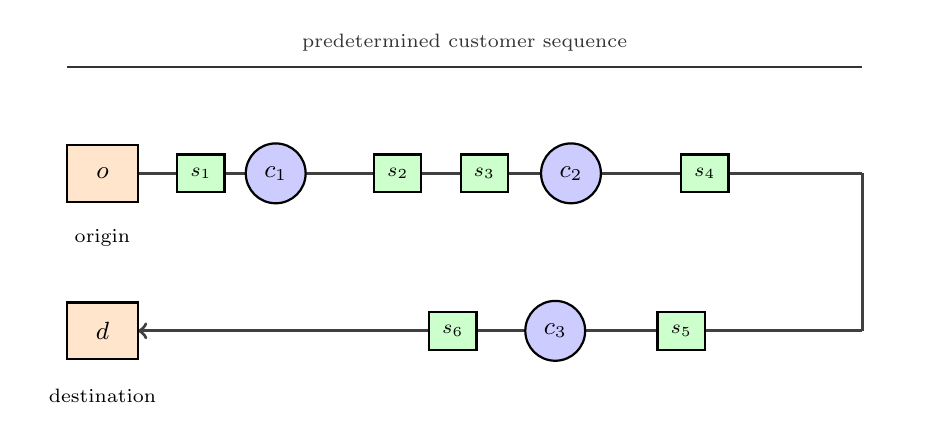
\begin{tikzpicture}[x=1cm,y=1cm]

% Fixed bounding box keeps the whole diagram geometrically centered
\path[use as bounding box] (-0.25,-2.95) rectangle (10.85,1.85);

% ===================== guide line =====================
% Aligned with the full horizontal extent of the route
\draw[thin,color=black!80]
    (0.25,1.35) --
    node[midway,above=2pt]
    {\scriptsize predetermined customer sequence}
    (10.35,1.35);

% ===================== route =====================
% Upper route
\draw[very thick,color=black!75]
    (1.15,0) -- (10.35,0);

% Downward turn
\draw[very thick,color=black!75]
    (10.35,0) -- (10.35,-2.0);

% Lower route, ending at destination
\draw[very thick,->,color=black!75]
    (10.35,-2.0) -- (1.15,-2.0);

% ===================== origin =====================
\draw[thick,fill=orange!20]
    (0.25,-0.36) rectangle (1.15,0.36);
\node at (0.70,0) {\small $o$};
\node at (0.70,-0.82) {\scriptsize origin};

% ===================== destination =====================
\draw[thick,fill=orange!20]
    (0.25,-2.36) rectangle (1.15,-1.64);
\node at (0.70,-2.0) {\small $d$};
\node at (0.70,-2.82) {\scriptsize destination};

% ===================== upper-row customers =====================
\draw[thick,fill=blue!20] (2.90,0) circle (0.38);
\node at (2.90,0) {\small $c_1$};

\draw[thick,fill=blue!20] (6.65,0) circle (0.38);
\node at (6.65,0) {\small $c_2$};

% ===================== upper-row charging stations =====================
\draw[thick,fill=green!20]
    (1.65,-0.24) rectangle (2.25,0.24);
\node at (1.95,0) {\scriptsize $s_1$};

\draw[thick,fill=green!20]
    (4.15,-0.24) rectangle (4.75,0.24);
\node at (4.45,0) {\scriptsize $s_2$};

\draw[thick,fill=green!20]
    (5.25,-0.24) rectangle (5.85,0.24);
\node at (5.55,0) {\scriptsize $s_3$};

\draw[thick,fill=green!20]
    (8.05,-0.24) rectangle (8.65,0.24);
\node at (8.35,0) {\scriptsize $s_4$};

% ===================== lower-row customer =====================
\draw[thick,fill=blue!20] (6.45,-2.0) circle (0.38);
\node at (6.45,-2.0) {\small $c_3$};

% ===================== lower-row charging stations =====================
% Travel direction on the lower row is from right to left:
% s5 -> c3 -> s6 -> d
\draw[thick,fill=green!20]
    (7.75,-2.24) rectangle (8.35,-1.76);
\node at (8.05,-2.0) {\scriptsize $s_5$};

\draw[thick,fill=green!20]
    (4.85,-2.24) rectangle (5.45,-1.76);
\node at (5.15,-2.0) {\scriptsize $s_6$};

\end{tikzpicture}

\caption{Illustrative route structure for the EVTDSP. The truck travels
from origin $o$ to destination $d$ through a predetermined sequence of
customers $(c_1,c_2,c_3)$, with charging stations $(s_1,\ldots,s_6)$
available along the route.}
\label{fig:evtdsp_route}
\end{figure}
%Let the predetermined route be represented by the ordered sequence of mandatory locations $\mathcal{R}=(c_0,c_1,\ldots,c_N,c_{N+1})$, where $c_0$ denotes the origin, $c_{N+1}$ the destination, and the intermediate locations correspond to customer visits. Consecutive locations $(c_i,c_{i+1})$ define route legs. Moreover, let $\mathcal{L}$ denote the set of all route \emph{legs}, i.e., $\mathcal{L}=\left\{(c_i,c_{i+1}) \mid i=0,\ldots,N-1\right\}$. Charging stations may be located along a leg. Let $\mathcal{P}$ denote the ordered set of physical nodes obtained by inserting all charging stations into the route. Consequently, each {leg} may be decomposed into one or more \emph{sublegs} connecting consecutive physical nodes in $\mathcal{P}$.
%\red{introduce a short table with notation? There are some things in the paper not defined.}

Each customer node $i \in \mathcal{N}^C$ has a fixed and uninterruptible service time $s_i$, while all charging nodes $i \in \mathcal{N}^S$ have a homogeneous charging rate $??$ denoting the amount of energy added to the battery per time unit of charging. Furthermore, each arc $(i,j) \in \mathcal{A}$ has a parameter $t_{ij}$ and $???$, denoting the amount of time and energy used to traverse the arc, respectively.  
The vehicle is equipped with a battery of fixed capacity, denoted $B$, %, measured in kwH 
and may recharge, either partially or fully, at any number of charging stations located along the route. 

The driver is subject to EU HoS regulations, which define allowable driving and working durations, as well as mandatory break and rest periods. Driving time includes only the operation of the vehicle between locations, while working time encompasses both driving and service time at customers. A break is a pause of at least $t_{break}$ hours required after a maximum of $t_{\texttt{drive}|B}$ hours of driving or $t_{\texttt{elapsed}|B}$ hours of total working time. A daily rest is an uninterrupted period of at least $t_{rest}$ hours required after a maximum of $t_{\texttt{drive}|R}$ hours of driving or $t_{\texttt{elapsed}|R}$ hours of total working time. 
Breaks and daily rests cannot be scheduled during customer service but may be taken at customer locations, charging stations, or intermediate points along the route. If a break or a daily rest is taken at a charging station, it may be synchronized with charging the vehicle. 
The objective is to determine the minimal possible route duration, while adhering to the HoS regulations, and ensuring that there is sufficient power in the vehicle's battery.


Figure~\ref{fig:driver_schedule} illustrates a valid HoS-compliant schedule under these rules. While EU regulations provide additional flexibility through mechanisms such as split breaks %and reduced or split daily rests
, the base formulation focuses on standard 45-minute breaks and full 11-hour daily rests. Additional regulatory options can be incorporated within the proposed framework but are omitted to maintain focus on the core scheduling problem. \red{REF to a goel paper doing more intricate HoS regulation?}


\begin{figure}[htbp!]
\centering
\resizebox{\textwidth}{!}{%


\begin{tikzpicture}
% Time blocks
\def\y{0}
\def\h{1}

% Drive: 4.5 hours
\fill[fill=lime!70] (0,\y) rectangle (4.5,\y+\h);
\node at (2.25,\y+0.5) {Drive};
\node at (2.25,\y-0.25) {4.5h};


% Break + Charge: 0.75 hours
\fill[fill=yellow!70] (4.5,\y) rectangle (5.25,\y+\h);
\node[font=\scriptsize, align=center] at (4.875,\y+0.5) {Break\\+\\Charge};
\node at (4.875,\y-0.25) {0.75h};

% Drive: 3 hours
\fill[fill=lime!70] (5.25,\y) rectangle (8.25,\y+\h);
\node at (6.75,\y+0.5) {Drive};
\node at (6.75,\y-0.25) {3h};

% Service: 2 hours
\fill[fill=gray!20] (8.25,\y) rectangle (10.25,\y+\h);
\node at (9.25,\y+0.5) {Service};
\node at (9.25,\y-0.25) {2h};

% Drive after service: 1.5 hours
\fill[fill=lime!70] (10.25,\y) rectangle (11.75,\y+\h);
\node at (11.0,\y+0.5) {Drive};
\node at (11.0,\y-0.25) {1.5h};

% Rest: 11 hours
\fill[fill=red!70] (11.75,\y) rectangle (22.75,\y+\h);
\node at (17.25,\y+0.5) {Rest};
\node at (17.25,\y-0.25) {11h};


\end{tikzpicture}%
}
\caption{Example of a schedule of a fully rested driver in accordance with EU HoS regulation.}
\label{fig:driver_schedule}
\end{figure}


%

    
    %------------------------------------------------%
    
    \section{ SPPRC Framework} 
    
    %------------------------------------------------%


The EVTDSP can be formulated as a shortest path problem with resource constraints (SPPRC) and solved using a labeling algorithm. Our modeling approach extends the parameter-free network and labeling framework of \citet{goel2017exact} to account for battery-electric truck operations. Feasibility is tracked through label resources representing elapsed time, Hours-of-Service counters, and battery-energy state. These resources are propagated through the network by resource extension functions (REFs) associated with the network arcs.
The framework supports both full- and partial-recharge strategies. We focus on the more general partial-recharge formulation, in which charging amounts are decision variables, while the full-recharge formulation is obtained as a special case and reported in \ref{app:full_recharge_spprc}. 

The remainder of this section first presents the underlying activity network, then introduces the label resources and REFs, and finally describes the feasibility and dominance rules used within the labeling algorithm.




\subsection{Parameter-free network structure}
%The SPPRC formulation is based on the parameter-free activity network of \citet{goel2017exact}, extended to incorporate charging-station visits. 
Charging stations are introduced as additional physical nodes along the route, so that a leg between two mandatory locations may be decomposed into several consecutive sublegs. Figure~\ref{fig:subnetwork_cs_partial} illustrates a route segment from customer $n$ to customer $m$ with a single intermediate charging station $s$, resulting in the sublegs $(n,s)$ and $(s,m)$.


\begin{figure}[htbp!]
\centering
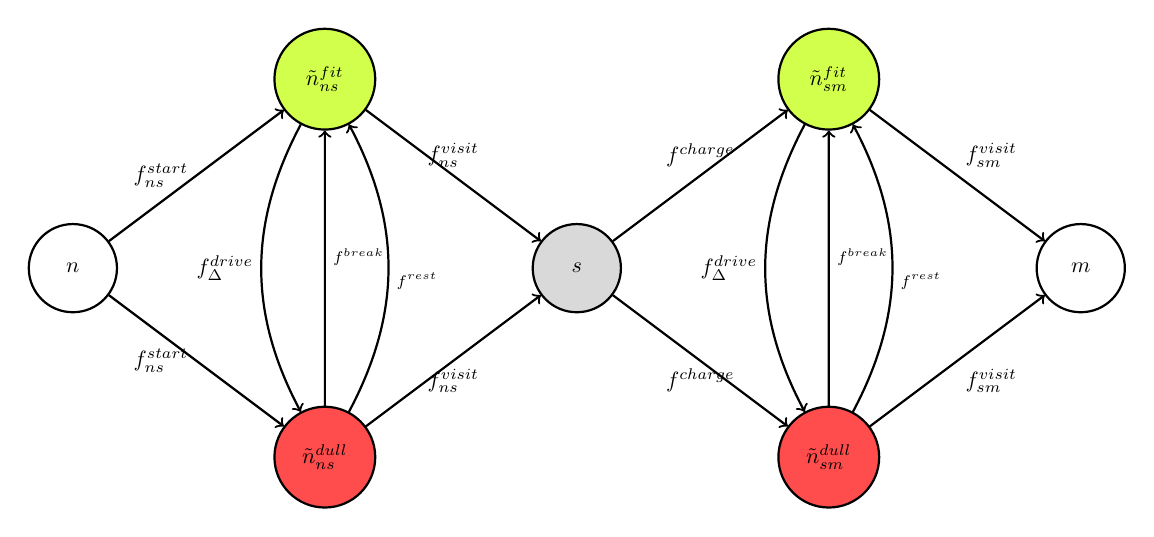
\begin{tikzpicture}[scale=0.8, transform shape, ->, thick, auto]
% Node styles
\tikzstyle{main} = [circle, draw=black, minimum size=1.4cm, inner sep=0pt]
\tikzstyle{fit}  = [circle, draw=black, fill=lime!70, minimum size=1.6cm, inner sep=0pt]
\tikzstyle{dull} = [circle, draw=black, fill=red!70, minimum size=1.6cm, inner sep=0pt]
\tikzstyle{cs}   = [circle, draw=black, fill=gray!30, minimum size=1.4cm, inner sep=0pt]

% Nodes
\node[main] (n) at (0,0) {$n$};
\node[fit]  (fitL) at (4, 3) {$\tilde{n}^{\text{fit}}_{ns}$};
\node[dull] (dullL) at (4, -3) {$\tilde{n}^{\text{dull}}_{ns}$};
\node[cs]   (cs) at (8, 0) {$s$};
\node[fit]  (fitR) at (12, 3) {$\tilde{n}^{\text{fit}}_{sm}$};
\node[dull] (dullR) at (12, -3) {$\tilde{n}^{\text{dull}}_{sm}$};
\node[main] (m) at (16,0) {$m$};

% From n to left states
\path (n) edge node[left] {$f^{\text{start}}_{ns}$} (fitL);
\path (n) edge node[left] {$f^{\text{start}}_{ns}$} (dullL);

% Transitions between fit/dull (left side)
\path[bend right=28] (fitL) edge node[left] {$f^{\text{drive}}_{\Delta}$} (dullL);
\path (dullL) edge node[right, yshift=5pt] {\scriptsize $f^{\text{break}}$} (fitL);
\path[bend right=28] (dullL) edge node[right, yshift=-6pt] {\scriptsize $f^{\text{rest}}$} (fitL);

% To s
\path (fitL) edge node[above] {$f^{\text{visit}}_{ns}$} (cs);
\path (dullL) edge node[below] {$f^{\text{visit}}_{ns}$} (cs);

% From s to right states
\path (cs) edge node[above] {$f^{\text{charge}}$} (fitR);
\path (cs) edge node[below] {$f^{\text{charge}}$} (dullR);

% Transitions between fit/dull (right side)
\path[bend right=28] (fitR) edge node[left] {$f^{\text{drive}}_{\Delta}$} (dullR);
\path (dullR) edge node[right, yshift=5pt] {\scriptsize $f^{\text{break}}$} (fitR);
\path[bend right=28] (dullR) edge node[right, yshift=-6pt] {\scriptsize $f^{\text{rest}}$} (fitR);

% From right states to m
\path (fitR) edge node[above right] {$f^{\text{visit}}_{sm}$}  (m);
\path (dullR) edge node[below right] {$f^{\text{visit}}_{sm}$} (m);
\end{tikzpicture}
\caption{Extended subnetwork with an intermediate charging station $s$ under the partial-recharge strategy. Arcs define resource extension functions.}
\label{fig:subnetwork_cs_partial}
\end{figure}



Each subleg between two consecutive physical nodes \(n\) and \(m\) is represented by an activity subnetwork containing two intermediate states, denoted by \(\tilde{n}_{nm}^{\mathrm{fit}}\) and \(\tilde{n}_{nm}^{\mathrm{dull}}\). The \emph{fit} state represents a situation in which the driver is allowed to continue driving, either because no break or daily rest is currently due or because the required one has just been completed. The \emph{dull} state represents a situation in which the driver must first take a break or daily rest before additional driving is permitted. Arcs between these states correspond to elementary driver activities, namely starting a leg, driving, taking a break, taking a daily rest, visiting the next physical node, and recharging at a charging station.

At a charging-station node, the schedule may initiate a charging activity. 
%Under the partial-recharge strategy, the amount of energy charged is a decision variable rather than being fixed to a full recharge. 
Charging is represented through recharge arcs originating from the charging-station node, allowing the schedule to continue after recharging with different battery-energy levels. 

The resulting network contains six classes of arcs: start arcs, driving arcs, break arcs, rest arcs, visit arcs, and recharge arcs. A key feature of this representation is that a driving arc is not assigned a fixed duration in advance. Instead, its duration \(\Delta\) is computed as the longest feasible driving duration given the current resource state.
%, equal to the minimum of (i) the remaining travel time to the next physical node, (ii) the remaining driving time until a mandatory break or daily rest, (iii) the remaining daily working time before a mandatory rest must begin, and (iv) the remaining driving time permitted by the available battery energy. 
Consequently, each driving extension terminates either at the next physical node or at the point where HoS or energy constraints require a new decision.



\subsection{Labeling algorithm}

We solve the SPPRC using a labeling algorithm. The algorithm starts with an initial label at the origin, representing a fully rested driver and a fully charged vehicle. At each iteration, an unprocessed label is extended along every outgoing arc that is feasible given its current resource state. The corresponding resource extension function (REF) updates the temporal, regulatory, and energy resources. Labels violating an HoS or battery constraint are discarded, while dominance rules eliminate labels that cannot lead to a better feasible completion than another label at the same node. A complete schedule is obtained when a label reaches the destination. 


\subsubsection{Label definition}


A label represents a partial path from the origin to the current network node, together with the resource state needed to assess its feasibility and extend it into a complete schedule. Formally, a label is represented by
\[
\mathcal{L}=(v,\pi,\mathbf{T}),
\]
where \(v\) is the current network node, \(\pi\) stores the predecessor information required to reconstruct the partial path, and \(\mathbf{T}\) contains its associated resources.

The resource vector includes the elapsed schedule time (\(\texttt{time}\)); the remaining driving time to the next physical node (\(\texttt{timeToNext}\)); the driving time since the last daily rest (\(\texttt{drive|R}\)); the driving time since the last break or daily rest (\(\texttt{drive|B}\)); the elapsed time since the end of the last daily rest (\(\texttt{elapsed|R}\)); the elapsed time since the end of the last break or daily rest (\(\texttt{elapsed|B}\)); and the vehicle's state of charge (\(\texttt{SOC}\)). The first six resources describe the temporal and HoS state of the partial schedule, while \(\texttt{SOC}\) describes its energy state.
%The HoS resources build on \citet{goel2017exact}. We additionally retain the break-specific resources \(\texttt{drive|B}\) and \(\texttt{elapsed|B}\), as both can become binding in our problem. 
%The energy deficit, when needed, is derived as \(\texttt{reqEC}:=B-\texttt{SOC}\). 
Table~\ref{tab:resource_windows_partial} summarizes the resources and their feasibility windows.



%A label \(l\) represents a partial path from the origin to a network node together with the temporal, regulatory, and energy information required to continue that partial schedule. The label maintains resources describing the elapsed time, remaining travel requirements, Hours-of-Service status, and battery energy.



\begin{table}[!htbp]
\centering
\caption{Label resources with corresponding feasibility windows.}
\label{tab:resource_windows_partial}
\begin{tabular}{@{}llll@{}}
\toprule
\textbf{Resource} & \textbf{Type} & \textbf{Description} & \textbf{Feasibility Window} \\
\midrule
$\texttt{time}$ & Temporal & Total time elapsed since departure & $[0,T_{\text{horizon}}]$ \\
$\texttt{timeToNext}$ & Temporal &  Remaining driving time to next physical node & $[0,t_{nm}]$ \\
$\texttt{drive|R}$ & Regulatory & Driving time since last daily rest & $[0,t_{\texttt{drive}|R}]$ \\
$\texttt{drive|B}$ & Regulatory & Driving time since last break or rest & $[0,t_{\texttt{drive}|B}]$ \\
$\texttt{elapsed|R}$ & Regulatory & Elapsed time since last daily rest & $[0,t_{\texttt{elapsed}|R}]$ \\
$\texttt{elapsed|B}$ &  Regulatory & Elapsed time since last break or rest & $[0,t_{\texttt{elapsed}|B}]$ \\
$\texttt{SOC}$ & Energy & Remaining battery energy (state of charge)
  & $[0,\,B]$ \\
\bottomrule
\end{tabular}
\end{table}

Under partial recharge, the amount of energy charged is a decision variable. Because charging time is linear in the amount of energy added, the feasible temporal and energy states can be represented by their interval endpoints, following interval-based representations in the literature (e.g., \citet{desaulniers2016exact}). Accordingly, \(\texttt{time}\) and \(\texttt{SOC}\) are represented by
\([l_{\texttt{time}}^{\min},l_{\texttt{time}}^{\max}]\) and
\([l_{\texttt{SOC}}^{\min},l_{\texttt{SOC}}^{\max}]\), respectively, while the HoS-related resources remain scalar-valued. The resulting resource vector is
\[
\mathbf{T}=
\bigl(
l_{\texttt{time}}^{\min},
l_{\texttt{time}}^{\max},
l_{\texttt{timeToNext}},
l_{\texttt{drive|R}},
l_{\texttt{drive|B}},
l_{\texttt{elapsed|R}},
l_{\texttt{elapsed|B}},
l_{\texttt{SOC}}^{\min},
l_{\texttt{SOC}}^{\max}
\bigr).
\]


%Dominance and label extension are defined with respect to labels ending at the same node $v$; resource comparisons therefore apply only among labels stored at that node.

%Feasibility of each label extension is enforced by requiring all resource components to remain within their prescribed bounds with respect to labels ending at the same node $v$. Under partial recharge, the resource windows given in Table~\ref{tab:resource_windows_partial} apply componentwise to the corresponding interval endpoints. 




\subsubsection{Resource extension functions}





%Each arc \(a = (i,j) \in A\) of the parameter-free network is associated with a resource extension function (REF) which maps a feasible label $\mathcal{L}=(v,\pi,\mathbf{T})$ at tail node $i$ to a new label $\mathcal{L}'=f_a(\mathcal{L})$ at head node $j$. 
Each arc \(a=(i,j)\in A\) is associated with a REF \(f_a\), which computes the resource vector \(\mathbf{T}'=f_a(\mathbf{T})\), or valid lower bounds on its components. %, at head node \(j\) from the resource vector \(\mathbf{T}\) at tail node \(i\). 
Extending a label \(\mathcal{L}=(i,\pi,\mathbf{T})\) along arc \(a\) then produces the label \(\mathcal{L}'=(j,\pi',\mathbf{T}')\), where \(\pi'\) contains the updated predecessor information. Furthermore, \(l'_r\) denotes the value of resource \(r\) after an extension, while \(l_r\) denotes its value before the extension.

The activity network uses six REFs: \(f^{\text{start}}_{ij}\), \(f^{\text{drive}}_{\Delta}\), \(f^{\text{break}}\), \(f^{\text{rest}}\), \(f^{\text{visit}}_{ij}\), and \(f^{\text{charge}}_i\). The first five build on the parameter-free framework of \citet{goel2017exact}. The temporal and HoS REFs are retained, while the driving REF is augmented to account for battery consumption. The recharge REF is introduced to model charging at charging stations.

The start REF initializes a subleg by setting the remaining travel time to \(t_{ij}\). The drive REF advances the schedule by a duration \(\Delta\), updating time, HoS counters, and battery energy. The break and rest REFs add the corresponding interruption and reset the applicable HoS counters. The visit REF records arrival at physical node \(j\) and, if \(j\) is a customer, adds the service time \(s_j\).

The duration of a driving extension is determined endogenously as
\[
\Delta = \min\Bigl\{
l_{\text{timeToNext}},
t_{R}^{\text{drive}}-l_{\text{drive|R}},
t_{B}^{\text{drive}}-l_{\text{drive|B}},
t^{\text{day}}-\bigl(l_{\text{elapsed|R}}+t_{\text{rest}}\bigr)
\Bigr\},
\]
Thus, a driving extension ends when the next physical node is reached or when a break, daily rest, or daily working-time limit becomes binding. The drive REF reduces the SOC by \(\alpha\Delta\), and the extension is feasible only if the resulting SOC remains nonnegative.

Under partial recharge, \(f^{\text{charge}}_i\) propagates the interval-valued time and SOC resources. Charging may add any amount of energy up to a full recharge, with charging time proportional to the energy added at rate \(CP\). If charging overlaps with an admissible break or daily rest, only the unsynchronized charging time increases the schedule duration. Table~\ref{tab:ref_common_partial} summarizes the resulting resource updates.



\begin{table}[!htbp]
\caption{Resource updates for the REFs on subleg \(a=(i,j)\). A dash indicates that the corresponding resource remains unchanged. In the charge column, intervals give the updated lower and upper endpoints, respectively.}
\label{tab:ref_common_partial}
\centering
\small
\setlength{\tabcolsep}{2.5pt}
\renewcommand{\arraystretch}{1.15}
\resizebox{\linewidth}{!}{%
\begin{tabular}{@{}lcccccc@{}}
\toprule
\multirow{2}{*}{\makecell[l]{\textbf{Updated}\\\textbf{resource}}}
& \multicolumn{6}{c}{\textbf{Resource extension function}}\\
\cmidrule(lr){2-7}
& \(f^{\text{start}}_{ij}\)
& \(f^{\text{drive}}_{\Delta}\)
& \(f^{\text{break}}\)
& \(f^{\text{rest}}\)
& \(f^{\text{visit}}_{ij}\)
& \(f^{\text{charge}}_i\)\\
\midrule

\(l'_{\text{time}}\)
& ---
& \(l_{\text{time}}+\Delta\)
& \(l_{\text{time}}+t_{\text{break}}\)
& \(l_{\text{time}}+t_{\text{rest}}\)
& \(l_{\text{time}}+s_j\)
& \(\begin{cases}
  \left[l^{\min}_{\text{time}},
        l^{\max}_{\text{time}}\right]
    & \text{if }l_{\text{elapsed|R}}=0,\\[2pt]
  \left[
    l^{\min}_{\text{time}}
      +\max\{0,\tau^{\mathrm{full}}-t_{\text{break}}\},
    l^{\max}_{\text{time}}
  \right]
    & \text{if }l_{\text{elapsed|B}}=0,\\[2pt]
  \left[
    l^{\min}_{\text{time}},
    l^{\max}_{\text{time}}+\tau^{\mathrm{full}}
  \right]
    & \text{otherwise}.
\end{cases}\)
\\

\(l'_{\text{timeToNext}}\)
& \(t_{ij}\)
& \(l_{\text{timeToNext}}-\Delta\)
& ---
& ---
& ---
& \(t_{ij}\)
\\

\(l'_{\text{drive|R}}\)
& ---
& \(l_{\text{drive|R}}+\Delta\)
& ---
& \(0\)
& ---
& ---
\\

\(l'_{\text{drive|B}}\)
& ---
& \(l_{\text{drive|B}}+\Delta\)
& \(0\)
& \(0\)
& ---
& ---
\\

\(l'_{\text{elapsed|R}}\)
& ---
& \(l_{\text{elapsed|R}}+\Delta\)
& \(l_{\text{elapsed|R}}+t_{\text{break}}\)
& \(0\)
& \(l_{\text{elapsed|R}}+s_j\)
& \(\begin{cases}
  0
    & \text{if }l_{\text{elapsed|R}}=0,\\[2pt]
  l_{\text{elapsed|R}}+\tau^{\min}_{\text{add}}
    & \text{otherwise}.
\end{cases}\)
\\

\(l'_{\text{elapsed|B}}\)
& ---
& \(l_{\text{elapsed|B}}+\Delta\)
& \(0\)
& \(0\)
& \(l_{\text{elapsed|B}}+s_j\)
& \(\begin{cases}
  0
    & \text{if }l_{\text{elapsed|B}}=0,\\[2pt]
  l_{\text{elapsed|B}}+\tau^{\min}_{\text{add}}
    & \text{otherwise}.
\end{cases}\)
\\

\(l'_{\text{SOC}}\)
& ---
& \(l_{\text{SOC}}-\alpha\Delta\)
& ---
& ---
& ---
& \(\begin{cases}
  [B,B]
    & \text{if }l_{\text{elapsed|R}}=0,\\[2pt]
  [B,B]
    & \text{if }l_{\text{elapsed|B}}=0
      \text{ and }\tau^{\mathrm{full}}\leq t_{\text{break}},\\[2pt]
  \left[
    \min\{B,l^{\min}_{\text{SOC}}+CP\,t_{\text{break}}\},
    B
  \right]
    & \text{if }l_{\text{elapsed|B}}=0
      \text{ and }\tau^{\mathrm{full}}>t_{\text{break}},\\[2pt]
  \left[l^{\min}_{\text{SOC}},B\right]
    & \text{otherwise}.
\end{cases}\)
\\

\bottomrule
\end{tabular}%
}
\end{table}

%comment STEF


For arc $a=(i,j)$, $t_{ij}$ denotes the driving time from node $i$ to $j$, and $s_j$ denotes the service time at customer $j$. Parameters $t_{\text{break}}$ and $t_{\text{rest}}$ denote the mandatory break and daily-rest durations, respectively; $\alpha$ is the energy consumption rate; $B$ is battery capacity; and $CP$ is charging power. For the common REFs, each expression in the rows for $l_{\text{time}}$ and $l_{\text{SOC}}$ applies to both interval endpoints, unless the recharge column states otherwise. In the recharge column, comma-separated expressions denote the updates of $l^{\min}$ and $l^{\max}$, respectively. Let $e^{\max}:=B-l^{\min}_{\text{SOC}}$ and $\tau^{\mathrm{full}}:=e^{\max}/CP$. The added charging times in $f^{\text{charge}}_{i}$ are
\[
\tau^{\min}_{\mathrm{add}}=
\begin{cases}
0 & l_{\text{elapsed|R}} = 0,\\[2pt]
0 & l_{\text{elapsed|B}} = 0,\;
  \tau^{\mathrm{full}} \le t_{\text{break}},\\[2pt]
\max\!\bigl\{0,\, \tau^{\mathrm{full}} - t_{\text{break}}\bigr\}
  & l_{\text{elapsed|B}} = 0,\;
  \tau^{\mathrm{full}} > t_{\text{break}},\\[2pt]
0 & \text{otherwise},
\end{cases}
\qquad
\tau^{\max}_{\mathrm{add}}=
\begin{cases}
0 & l_{\text{elapsed|R}} = 0,\\[2pt]
0 & l_{\text{elapsed|B}} = 0,\;
  \tau^{\mathrm{full}} \le t_{\text{break}},\\[2pt]
\tau^{\mathrm{full}} - t_{\text{break}}
  & l_{\text{elapsed|B}} = 0,\;
  \tau^{\mathrm{full}} > t_{\text{break}},\\[2pt]
\tau^{\mathrm{full}} & \text{otherwise}.
\end{cases}
\]
The scalar full-recharge REFs in Table~\ref{tab:ref_full_recharge} are recovered when $l^{\min}=l^{\max}$ and each recharge extension performs a complete recharge, so that $\tau^{\mathrm{full}}=(B-l_{\text{SOC}})/CP$ and both interval endpoints coincide.


\subsubsection{Feasibility and dominance}

After each resource extension, the resulting label must remain feasible. Feasibility is enforced through the resource windows in Table~\ref{tab:resource_windows_partial}; labels violating any bound are discarded immediately. Under partial recharge, the windows for $\texttt{time}$ and $\texttt{SOC}$ apply to each interval endpoint. In addition, the activity network restricts which extensions are allowed at each state: from a \emph{dull} state, only break or rest arcs may be taken before driving resumes, whereas from a \emph{fit} state driving is allowed and, once $l_{\text{timeToNext}}=0$, visit or recharge arcs become available.

To limit the number of labels stored at each network node, dominance is applied among labels ending at the same node $v$. Let $\mathcal{L}_1=(v,\pi_1,\mathbf{T}_1)$ and $\mathcal{L}_2=(v,\pi_2,\mathbf{T}_2)$ be two feasible labels at node $v$. Label $\mathcal{L}_1$ dominates $\mathcal{L}_2$ if and only if:
\begin{align*}
l_{\text{timeToNext}}^{(1)} &\le l_{\text{timeToNext}}^{(2)}, \\
l_{\text{drive|R}}^{(1)} &\le l_{\text{drive|R}}^{(2)}, &
l_{\text{drive|B}}^{(1)} &\le l_{\text{drive|B}}^{(2)}, \\
l_{\text{elapsed|R}}^{(1)} &\le l_{\text{elapsed|R}}^{(2)}, &
l_{\text{elapsed|B}}^{(1)} &\le l_{\text{elapsed|B}}^{(2)}, \\
l_{\text{latest|R}}^{(1)} &\ge l_{\text{latest|R}}^{(2)}, &
l_{\text{latest|B}}^{(1)} &\ge l_{\text{latest|B}}^{(2)}, \\
l_{\text{time}}^{\min,(1)} &\le l_{\text{time}}^{\min,(2)}, \\
l_{\text{SOC}}^{\min,(1)} &\ge l_{\text{SOC}}^{\min,(2)}, &
l_{\text{SOC}}^{\max,(1)} &\ge l_{\text{SOC}}^{\max,(2)}.
\end{align*}

and, at the earliest departure time of label 2, label 1 must offer at least the same battery energy, accounting for optional charging between $l_{\text{time}}^{\min,(1)}$ and $l_{\text{time}}^{\max,(1)}$.  Since the objective is to minimize total route duration, a label is preferable if its resource values are at least as good for continuing the route. For the scalar HoS resources ($\texttt{timeToNext}$, $\texttt{drive|R}$, $\texttt{drive|B}$,
$\texttt{elapsed|R}$, and $\texttt{elapsed|B}$), which are monotone non-decreasing along every REF except break, rest, and synchronized recharge, label~1 dominates label~2 at the same node if each of these resources is no
larger in label~1 than in label~2. This pairwise comparison is sufficient for SPPRC with monotone resources and
preserves optimality \citep{irnich2005shortest, goel2017exact}. Resources $\texttt{latest|R}$ and $\texttt{latest|B}$ are compared in the reverse direction because larger values correspond to greater remaining scheduling flexibility. The partial-recharge extension introduces interval-valued time and SOC resources. The additional dominance conditions on $l_{\text{time}}^{\min}$, $l_{\text{SOC}}^{\min}$, $l_{\text{SOC}}^{\max}$, and the battery level at $t=l_{\text{time}}^{\min,(2)}$ follow the interval dominance rule for delivery paths with optional recharging
\citep{desaulniers2016exact}.

%When \(\bigl[l_{\text{time}}^{\min},\, l_{\text{time}}^{\max}\bigr]\) reduces to a single time value and \(\bigl[l_{\text{reqEC}}^{\min},\, l_{\text{reqEC}}^{\max}\bigr]\) reduces to a single energy value, these conditions simplify to the scalar full-recharge dominance rule reported in Appendix~\ref{app:full_recharge_spprc}.




    
    %------------------------------------------------%
    
    \section{Experimental design} %Experimental design
    
    %------------------------------------------------%


This section outlines the experimental design used in the computational study. We first describe the benchmark instances used to evaluate the proposed framework. We then introduce a baseline scheduling heuristic, which serves as a reference for assessing the benefits of jointly optimizing charging, breaks, and daily rests.

%------------------------------------------------%
\subsection{Benchmark instances}
%------------------------------------------------%


Long-haul freight operations vary substantially in route length, customer distribution, and operating conditions. These characteristics influence the potential gains from jointly scheduling charging, mandatory breaks, and daily rests. We therefore develop a diverse set of structural route instances and evaluate them under different charging-station coverage levels, battery capacities, charging powers, and energy-consumption rates. Rather than reproducing individual observed routes, the instances represent a broad range of realistic long-haul freight operations and constitute, to the best of our knowledge, the first benchmark set for the long-haul EVTDSP.

The benchmark design was informed by interviews with freight operators in Scandinavia and Northern Europe. With assistance from the Norwegian Trucking Association (NLF), 28 companies from different regions and transport segments were contacted, of which eight participated. They represented general freight, container, seafood, temperature-controlled, waste, and bulk transport. The interviews highlighted considerable variation in route length, route duration, number of stops, and customer distribution. Customers were often geographically clustered, resulting in routes that combine long intercity movements with shorter local collection and distribution activities. The interviews also emphasized the importance of charging-station availability and the potential gains from coordinating charging with mandatory driver breaks and daily rests.

\red{Include a pseudocode summarizing the procedure? }
Based on these industry inputs, we develop an instance generator for heterogeneous long-haul routes. The generator first defines route instances along three main dimensions: route length, customer distribution, and the number of customer stops. %These dimensions are represented through route, cluster, and customer classes, respectively. 
Scenario parameters are added subsequently to vary charging-station spacing, battery capacity, charging power, and energy consumption without changing the underlying route and customer structure.


Routes are classified as {short}, {medium}, or {long}, corresponding to increasing route distances. Specifically, short routes span 800--1200~km and typically require 1--2 overnight rests, while medium routes span 1500--2500~km and require 3--4 overnight rests. Long routes span 3000--4000~km and require 5--6 overnight rests, reaching the maximum multi-day operating horizon of six days before a longer weekly rest becomes necessary under the HoS regulations. For each instance, the total route length \(D_{\text{total}}\) is sampled uniformly from the interval associated with its route class.

Each route contains between one and three industrial clusters, interpreted as groups of geographically proximate customers. Cluster centers are positioned along intermediate sections of the route, so that customer visits are concentrated around these clusters and the first and last long-haul legs are typically the longest. %do not include this part: For a route of total length \(D_{\text{total}}\), the cluster centers are placed approximately at 50--60\% of \(D_{\text{total}}\) for one-cluster routes, at 35--45\% and 55--65\% for two-cluster routes, and at 25--30\%, 50--55\%, and 70--75\% for three-cluster routes. 
%Small perturbations of \(D_{\text{total}}\) are introduced to avoid artificial symmetry.


Customer stops are generated in two steps. First, one of three customer-count categories is selected: \textit{few} (1--3 customers), \textit{medium} (4--5 customers), or \textit{many} (6--15 customers), and the total number of customers \(N\) is sampled from the corresponding range. Second, customers are allocated among the route clusters, with at least one customer assigned to each cluster. In the base configurations, customers are distributed approximately evenly among clusters, refered to as balanced instances. For selected multi-cluster configurations, an unbalanced variant is also generated by assigning most customers to one randomly selected dominant cluster and only a few to the remaining clusters. For example, 12 customers across three clusters may be allocated as \([4,4,4]\) in a balanced instance and \([9,2,1]\) in an unbalanced instance. %The cluster centers remain distributed relatively evenly along the route in both variants, and the distinction does not apply to single-cluster routes. 

Customer locations are then placed within 75~km of their cluster center in either direction along the route, while maintaining local customer-to-customer distances of 30--150~km. This produces long intercity movements between clusters and shorter local movements within them. Service times are linked to the customer-count category: 20--30 minutes per stop for few-customer instances, 10--20 minutes for medium instances, and 5--10 minutes for many-customer instances. Instance names indicate the route class, number of clusters, number of customers, and, where applicable, the allocation variant; for example, \texttt{long\_cl2\_cu5\_Balanced}.


A total of \red{42} unique structural benchmark instances are generated by combining the route, cluster, and customer classes described above. Table~\ref{tab:benchmark_structure} summarizes the structural design, while the full set of instances and their characteristics is reported in Table~\ref{tab:test_instance_config}.

\begin{table}[!htbp]
\caption{Structural design of the benchmark instances.}
\label{tab:benchmark_structure}
\centering
\small
\setlength{\tabcolsep}{5pt}
\renewcommand{\arraystretch}{1.15}
\begin{tabular}{@{}lll@{}}
\toprule
\textbf{Characteristic} & \textbf{Class} & \textbf{Values} \\
\midrule
Route class
    & Short  & 800--1200 km (1--2 nights) \\
    & Medium & 1500--2500 km (3--4 nights) \\
    & Long   & 3000--4000 km (5--6 nights) \\
Clusters per route
    & Cluster class & 1--3 clusters \\
Customer class
    & Few    & 1--3 customers \\
    & Medium & 4--5 customers \\
    & Many   & 6--15 customers \\
Sampled customers
    & By route class & Short: 2--12; medium: 2--13; long: 2--14 \\
Service time per stop
    & Few    & 20--30 min \\
    & Medium & 10--20 min \\
    & Many   & 5--10 min \\
\red{Variants}
    & \red{Multi-cluster routes} & \red{Balanced; Unbalanced} \\
\bottomrule
\end{tabular}
\end{table}

Figure~\ref{fig:representative_routes} illustrates three representative instances. Charging stations are shown using the base-case maximum spacing of 50~km; the spacing parameter is defined below.

\begin{figure}[!htbp]
\centering

\begin{subfigure}[t]{0.90\textwidth}
    \centering
    \includegraphics[width=\linewidth]
    {figures/route_corridor_short_cl2_cu3_Balanced.pdf}
    \caption{\texttt{short\_cl2\_cu3\_Balanced}}
\end{subfigure}

\vspace{0.4em}

\begin{subfigure}[t]{0.90\textwidth}
    \centering
    \includegraphics[width=\linewidth]
    {figures/route_corridor_med_cl3_cu13_Balanced.pdf}
    \caption{\texttt{med\_cl3\_cu13\_Balanced}}
\end{subfigure}

\vspace{0.4em}

\begin{subfigure}[t]{0.90\textwidth}
    \centering
    \includegraphics[width=\linewidth]
    {figures/route_corridor_med_cl3_cu13_Unbalanced.pdf}
    \caption{\texttt{med\_cl3\_cu13\_Unbalanced}}
\end{subfigure}

\vspace{0.4em}

\begin{subfigure}[t]{0.90\textwidth}
    \centering
    \includegraphics[width=\linewidth]
    {figures/route_corridor_legend.pdf}
\end{subfigure}

\caption{Three representative benchmark instances illustrating variation in route length and customer distribution. Charging stations are shown using a maximum spacing of 50~km. \red{note: I found one instance where clusters  are overlapping -> mistake in instance generation? short cl2 cu4 Balanced}}
\label{fig:representative_routes}
\end{figure}


The computational experiments use different technological and infrastructure parameters, as summarized in Table~\ref{tab:scen_par}. 

\begin{table}[!htbp]
\caption{Scenario parameters and fixed HoS parameters.}
\label{tab:scen_par}
\centering
\small
\setlength{\tabcolsep}{5pt}
\renewcommand{\arraystretch}{1.15}
\begin{tabular}{@{}llll@{}}
\toprule
\multicolumn{4}{@{}l}{\textit{Scenario parameters}} \\
\textbf{Parameter} & \textbf{Symbol} &
\textbf{Base value} & \textbf{Sensitivity values} \\
\midrule
Battery capacity
    & \(B\) & 500 kWh & 350, 750 kWh \\
Charging power
    & \(P_{\text{ch}}\) & 350 kW & 1000 kW \\
Maximum charging-station spacing
    & \(d_{\text{CS}}\) & 50 km & 40, 60, \ldots, 100 km \\
Energy consumption
    & \(\alpha\) & 1.49 kWh/km & 1.12, 2.08 kWh/km \\

\addlinespace[0.6em]
\multicolumn{4}{@{}l}{\textit{Fixed HoS parameters}} \\
\textbf{Parameter} & \textbf{Symbol} &
\multicolumn{2}{l}{\textbf{Value}} \\
\midrule
Maximum continuous driving time
    & \(t_{\text{drive}|B}\) & \multicolumn{2}{l}{4.5 h} \\
Daily driving limit
    & \(t_{\text{drive}|R}\) & \multicolumn{2}{l}{9 h} \\
Maximum elapsed time before break
    & \(t_{\text{elapsed}|B}\) & \multicolumn{2}{l}{6 h} \\
Maximum elapsed time before daily rest
    & \(t_{\text{elapsed}|R}\) & \multicolumn{2}{l}{13 h} \\
Minimum break duration
    & \(t_{\text{break}}\) & \multicolumn{2}{l}{0.75 h} \\
Minimum daily rest duration
    & \(t_{\text{rest}}\) & \multicolumn{2}{l}{11 h} \\
\bottomrule
\end{tabular}
\end{table}

The selected battery capacities of 350, 500, and 750~kWh span current and announced heavy-duty electric-truck configurations, which range from approximately 360 to 780~kWh \citep{winkler2026potential,volvofhElectric,mercedesEactros600,volvo2025fhaero}. Charging powers of 350 and 1000~kW represent high-power CCS charging and prospective Megawatt Charging System capabilities, respectively. For example, the Mercedes-Benz eActros~600 supports up to 400~kW with CCS and 1000~kW with MCS \citep{mercedesEactros600}. In our model, these values are treated as constant charging rates; the 1000~kW case should therefore be interpreted as an idealized near-future scenario. Energy-consumption rates of 1.12, 1.49, and 2.08~kWh/km represent operating conditions ranging from favorable to demanding, around values reported in empirical studies and real-world trials \citep{volvofhElectric,le2025real}. Travel times are calculated using a fixed average speed of \red{60~km/h}, based on historical data provided by an industry partner.

The maximum charging-station spacing ranges from 40 to 100~km. This range reflects the 2030 targets in EU Regulation 2023/1804 (AFIR): publicly accessible charging sites for heavy-duty vehicles must be available in each direction of travel at intervals of at most 60~km along the TEN-T core network and 100~km along the comprehensive network; including at least two 350~kW charging points on the core network and one on the comprehensive network \citep{eu2023afir}.

Charging stations are inserted separately along each route leg. If a leg is shorter than the selected maximum spacing, one station is placed at its midpoint. Otherwise, stations are distributed such that the distance between consecutive charging opportunities does not exceed the selected spacing. The spacing parameter thus represents an upper bound rather than the exact distance between neighboring stations.

The HoS parameters are fixed across all experiments. Following \citet{goel2017exact}, we use maximum continuous and daily driving times of 4.5 and 9~h, maximum elapsed times of 6 and 13~h before a break and daily rest, and minimum break and daily-rest durations of 0.75 and 11~h, respectively. 



\begin{algorithm}[t]
\caption{Benchmark instance generation}
\label{alg:instance-generator}
\begin{algorithmic}[1]
\color{red}
\Require Route class $r$, number of clusters $K$, number of customers $N$,
         allocation type $a$, random seed
\Ensure Instance data, distance matrix, time matrix, and diagnostics

\State Sample the total route length $D$ according to route class $r$
\State Place $K$ cluster centers approximately evenly along $[0,D]$,
       with small random perturbations
\If{$K=1$}
    \State Assign all customers to the single cluster
\ElsIf{$a=\textsc{Balanced}$}
    \State Distribute the $N$ customers approximately evenly among the clusters
\Else
    \State Select one dominant cluster at random
    \State Assign most customers to the dominant cluster and only a few to each remaining cluster
\EndIf
\State Sample customer positions around their assigned cluster centers
\State Adjust customer positions to satisfy the required spacing constraints
\State Construct the predetermined visit sequence from the origin through the customers to the destination
\State Compute pairwise route distances $d_{ij}$
\State Compute travel times as $t_{ij} \gets d_{ij}/60$, assuming a constant speed of $60$ km/h
\State Generate customer service times %and time windows
\If{the feasibility conditions are violated}
    \State Resample the instance until a feasible configuration is obtained
\EndIf
\State Write the instance file, distance and time matrices, and diagnostic data
\end{algorithmic}
\end{algorithm}




\begin{comment}
After generating the structural route instances, we combine each route with scenario parameters. These parameters vary the availability of chargers along the route through the charging-station spacing, as well as battery capacity, charging power, and energy consumption. The parameter ranges are chosen to span both currently available heavy-duty battery-electric truck technologies and plausible near-future developments in vehicle and charging capabilities. Battery capacity ranges from 480 to 624 kWh, with an average of 540 kWh \citep{winkler2026potential}. Energy consumption is set to 1.15 kWh/km, with a variation of  $\pm$0.15 kWh/km to account for different driving conditions and loads \citep{le2025real}. \red{REFS to reports for battery capacity, charging power, and energy-consumption ranges, if possible @mostafa/@Odd-Andre}.
INPUT: Have not found any useful references for this, but as an example, the eActros 600 is reported to have a chrging power of 400 kW for CCS2 and 1000 kW for MCS. These are maximum values, but from the data I have seen, the charging curves with CCS2 are relatively constant just below the max value of 400 kW. Not sure how to address this in the paper. I think the most realistic base value woud be 400 kW, and if necesary refer to the CCS standard from Charin.
The average driving speed is fixed to \red{XXkmh -> Mostafa.} across all instances based on historical data provided by one of the industry partners. \red{should we use le2025real instead (41km/h -> I do not think so, seems too slow for our setting.}

Charging stations are inserted along each route leg based on the selected charging-station spacing parameter. The range of spacing values is based on regulatory targets for publicly available charging infrastructure for heavy-duty vehicles under Regulation (EU) 2023/1804 (AFIR), which states that by December 2030, recharging pools must be deployed in each direction of travel with a maximum distance of 60 km between them along the TEN-T core road network. For the TEN-T comprehensive road network, the maximum distance is 100 km \citep{eu2023afir}. \red{REF to some EU report stating min required distance between charging stations. } .

If a route leg is shorter than the specified spacing, a single charging station is placed at its midpoint. Otherwise, multiple charging stations are distributed along the leg such that the distance between consecutive charging opportunities does not exceed the specified spacing. Consequently, the charging-station spacing should be interpreted as a maximum spacing level rather than an exact distance between neighboring stations. Table~\ref{tab:benchmark_design} summarizes the instance classes, scenario values, and fixed HoS parameters used throughout the experiments.

\red{Other parameters which are forgotten / not defined?}


% Each route is represented as a linear sequence of nodes,
% \[
% \text{Origin} \rightarrow \text{Customer}_1 \rightarrow \cdots \rightarrow \text{Customer}_N \rightarrow \text{Destination},
% \]
% with cumulative distances satisfying \(\sum_i \Delta d_i = D_{\text{total}}\) and \(\Delta d_i>0\). Travel times are derived from these distances using a constant average speed consistent with the optimization model. The resulting distance and travel-time data populate the \texttt{DistanceMatrix.csv} and \texttt{TimeMatrix.csv} files used by the network parser to construct arcs between consecutive physical nodes.

\end{comment}






%------------------------------------------------%
\subsection{Baseline heuristic: sequential scheduling}
\label{sec:baseline_heuristic}
%------------------------------------------------%


We compare the proposed labeling-based approach against a sequential scheduling heuristic. The heuristic is designed to mimic how a driver or dispatcher might plan a fixed itinerary by making decisions incrementally along the route rather than jointly optimizing all charging and HoS decisions. Given a predefined customer sequence %$c_1 \rightarrow c_2 \rightarrow \dots \rightarrow c_N$
, the heuristic constructs a feasible schedule by progressing through the route one leg at a time. For each leg, the heuristic determines whether charging, a mandatory break, or a daily rest is required before continuing. Charging decisions are guided by a battery safety margin and a one-step look-ahead that considers the energy requirements of the subsequent route segment. When charging is required, the heuristic identifies the furthest charging station that can be reached safely on the current leg and charges the vehicle to full capacity. Mandatory breaks and daily rests are inserted whenever required by Hours-of-Service (HoS) regulations, and are synchronized with charging activities whenever both occur at the same charging station. The heuristic is computationally inexpensive and yields feasible schedules using only local route information, making it a useful benchmark for evaluating the benefits of joint optimization. The detailed scheduling logic is described below.

For each customer-to-customer leg $(A \rightarrow B)$, the scheduler first evaluates whether the current SoC can cover the required energy $E(A!\rightarrow!B)$ while maintaining a safety buffer equal to 30\% of battery capacity. A one-step look-ahead is then applied. The vehicle proceeds directly to $B$ if the remaining SoC upon arrival is sufficient either to: (i) complete the next leg $(B \rightarrow C)$ while maintaining the same safety buffer; or (ii) reach a charging station on the leg $(B \rightarrow C)$. Otherwise, the algorithm selects the furthest reachable charging station on $(A \rightarrow B)$, drives there, and recharges the vehicle to full capacity before continuing. If no charging station is reachable on the current leg, the algorithm backtracks to the most recent charging station on the previous leg and revises the schedule accordingly.

HoS constraints are enforced by evaluating each planned route leg against the current break and rest counters. If a mandatory break or daily rest would be due before the leg can be completed, the corresponding interruption (45 minutes or 11 hours, respectively) is inserted. When a stop occurs at a charging station, the scheduler \emph{synchronizes} charging and HoS: it overlaps the required break/rest with the ongoing charge and adds only the excess duration beyond the charging time to the route. The one-step look-ahead used for synchronization also considers the time to the first CS on the next arc, ensuring due stops are anticipated rather than deferred. %This logic is illustrated in Figure~\ref{fig:greedy_scheduler}, where a sample route shows charging stops aligned with driver breaks. 
The full procedure is given in Algorithm~\ref{alg:myopic}.

\begin{algorithm}[H]
{\color{red}
\caption{Sequential scheduling heuristic}
\label{alg:myopic}
\small
\begin{algorithmic}[1]
\Require Predetermined route $\mathcal{R}=(c_0,\ldots,c_{N+1})$, leg set
$\mathcal{L}=\left\{(c_i,c_{i+1}) \mid i=0,\ldots,N\right\}$ 
%,charging stations along each leg
%\Ensure Feasible schedule with total duration $T$, or \textsc{Infeasible}

\State Initialize SoC to full battery capacity, reset all HoS counters, and set $T\leftarrow 0$

\For{each leg $(c_i,c_{i+1})\in\mathcal{L}$}

    \State Check whether the vehicle can reach $c_{i+1}$ while maintaining the safety SoC margin

    \If{the leg can be completed safely}
        \State Apply one-step look-ahead from $c_{i+1}$
        \If{the remaining SoC at $c_{i+1}$ is sufficient to reach $c_{i+2}$ or reach a charging station on leg $(c_{i+1}, c_{i+2})$}
            \State Drive to $c_{i+1}$
        \Else
            \State Select the furthest reachable charging station on $(c_i,c_{i+1})$
            \State Drive to the selected charging station and charge to full capacity
            \State Continue to $c_{i+1}$
        \EndIf
    \Else
        \If{a charging station on $(c_i,c_{i+1})$ is reachable}
            \State Select the furthest reachable charging station on $(c_i,c_{i+1})$
            \State Drive to the selected charging station and charge to full capacity
            \State Continue toward $c_{i+1}$
        \ElsIf{backtracking to the most recent charging station yields a feasible continuation}
            \State Revise the previous leg by charging at the most recent charging station
            \State Retry leg $(c_i,c_{i+1})$
        \Else
            \State \Return \textsc{Infeasible}
        \EndIf
    \EndIf

    \State Insert any mandatory break or daily rest required before completing the planned driving
    \State If the interruption occurs at a charging station, overlap charging and HoS interruption whenever possible
    \State Apply service at $c_{i+1}$ if $c_{i+1}$ is a customer
    \State Update SoC, HoS counters, and total duration $T$

\EndFor

\State \Return $T$
\end{algorithmic}
}
\end{algorithm}


\begin{algorithm}[H]
{\color{red}
\caption{Sequential myopic scheduling heuristic}
\label{alg:myopic_alt}
\small
\begin{algorithmic}[1]
% \Require Fixed route $\mathcal{R} = (A_1,\ldots,A_N)$; CS locations on each arc;
%          battery capacity $B$; safety fraction $\beta$; consumption rate $\alpha$;
%          charging power $CP$; HoS limits $(T^{\max}_{\text{drive|B}}, T^{\max}_{\text{drive|R}},
%          T^{\max}_{\text{elapsed|B}}, T^{\max}_{\text{elapsed|R}})$;
%          minimum stop durations $(t_{\text{break}}, t_{\text{rest}})$
% \Ensure Feasible schedule with total time $T$ (or \textsc{Infeasible})
\State Initialize SoC $\leftarrow B$, HoS counters, $T \leftarrow 0$
\For{each arc $(A \rightarrow B)$ in $\mathcal{R}$}
    \State $E_{AB} \leftarrow \alpha \cdot d(A,B)$;\quad $b \leftarrow \beta B$
    \State \textbf{Onward look-ahead:} compute required $\rho_B$ on $B\!\rightarrow\!C$
           (energy to next leg or to furthest CS on $B\!\rightarrow\!C$, plus $b$)
    \If{SoC $\geq E_{AB} + b$ \textbf{and} SoC $- E_{AB} \geq \rho_B$}
        \State \Call{Drive}{$A,B$};\quad apply service at $B$ if applicable
    \ElsIf{SoC $\geq E_{AB} + b$ \textbf{and} a CS on $B\!\rightarrow\!C$ is reachable after $B$}
        % \State \Call{Drive}{$A,B$} \Comment{defer charging; handle $B\!\rightarrow\!C$ next iteration}
    \ElsIf{a CS on $A\!\rightarrow\!B$ is reachable with current SoC}
        \State $s^\ast \leftarrow$ furthest reachable CS on $A\!\rightarrow\!B$
        \State \Call{Drive}{$A,s^\ast$};\quad \Call{ChargeToFull}{}
        \State \Call{DriveWithHoSSync}{$s^\ast,B$};\quad apply service at $B$
    \ElsIf{a CS exists on the previous arc}
        \State backtrack, recharge at last CS, return to $A$, then retry leg
    \Else
        \State \Return \textsc{Infeasible}
    \EndIf
    \State Update HoS counters after each drive and service activity
\EndFor
\State \Return $T$
\Procedure{Drive}{$u,v$}
    \If{HoS limits violated before reaching $v$}
        \State insert $t_{\text{break}}$ or $t_{\text{rest}}$; reset counters
    \EndIf
    \State $T \leftarrow T + d(u,v)/v_{\text{speed}}$;\quad SoC $\leftarrow$ SoC $- \alpha\,d(u,v)$
\EndProcedure
\Procedure{DriveWithHoSSync}{$u,v$}
    \If{break/rest due within drive to $v$ (incl.\ look-ahead to first CS on next arc)}
        \State overlap stop with charging; $T \leftarrow T + \max\{0,\, t_{\text{stop}} - t_{\text{charge}}\}$
    \EndIf
    \State execute drive $u \rightarrow v$ and update counters
\EndProcedure
\end{algorithmic}
}
\end{algorithm} 




\begin{comment}
\begin{figure}[h!]
    \centering
    \includegraphics[width=0.9\textwidth]{figures/Greedy_Figure.png}
    \caption{Illustration of the greedy arc-feasibility logic. A link is retained only if the route can continue from the next node; otherwise, recharging is inserted at the farthest reachable charging station. HoS feasibility and charging synchronization are checked at each decision point.}


    \label{fig:greedy_scheduler}
\end{figure}
\end{comment}






    %------------------------------------------------%
    \section{Computational results} \label{sec:Computational Results}
    %------------------------------------------------%



This section reports the computational results. We first compare partial recharge, full recharge, the greedy heuristic, and the diesel proxy in the base-case setting. We then examine how these differences vary across instance classes and relate them to charging synchronization. Finally, we analyze the sensitivity of the results to battery characteristics, charging infrastructure, and energy consumption.

\subsection{Performance comparison of charging strategies}  %what

Table~\ref{tab:base_case_overview} summarizes the aggregate benchmark comparison for the base-case scenario. The results indicate that the dominant performance effect comes from optimization itself: schedules produced by the exact methods substantially outperform the greedy benchmark, highlighting the benefit of jointly optimizing charging decisions and driver scheduling under the Hours-of-Service regulation. Within this optimized setting, partial recharge provides a further systematic improvement over full recharge, indicating that additional value comes from adjusting charging amounts more precisely to downstream scheduling opportunities.
\begin{table}[!htbp]
\centering
\caption{Base-case comparison: partial recharge vs.\ alternative solution approaches.}
\label{tab:base_case_overview}
\begin{threeparttable}
\begin{tabular}{l r r r r r r r}
\toprule
Alternative &
$n$ &
\multicolumn{2}{c}{Mean route time (h)} &
\multicolumn{4}{c}{Partial advantage (benchmark $-$ partial)} \\
\cmidrule(lr){3-4} \cmidrule(lr){5-8}
& &
Partial & Alternative &
Mean (\%) & Mean (min) & Min (min) & Max (min) \\
\midrule
Full recharge & 43 & 81.93 & 82.43  &  0.61 &  29.95 &   4.80 &  89.39 \\
Greedy        & 42 & 83.14 & 119.15 & 28.83 & 2160.35 &  56.07 & 4225.01 \\
Diesel proxy  & 43 & 81.93 &  81.30 & $-$0.71 & $-$37.55 & $-$180.00 & 0.00 \\
\bottomrule
\end{tabular}
\begin{tablenotes}[flushleft]
\footnotesize
\item Each row compares partial recharge with one alternative on the same test instances ($n$). Partial advantage: positive values mean partial recharge is faster. Min/Max (min) are the smallest and largest instance-level time differences in minutes.
% \item Mean route times are averaged over those matched instances only (hence partial means differ across rows).
% \item Partial advantage: positive values mean partial recharge is faster; negative values mean the alternative is faster.
% \item Min/Max (min) are the smallest and largest instance-level time differences in minutes.
\end{tablenotes}
\end{threeparttable}
\end{table}

At the same time, the small average gap to the diesel reference case suggests that, when charging is coordinated effectively with mandatory breaks and daily rests, battery-electric operation can come close to diesel-like performance in the base-case setting. This average result is not uniform across instances, however. Figure~\ref{fig:base_case_per_instance} shows that the advantage of partial recharge over full recharge varies across the test set, and that the remaining EV--diesel gap is concentrated in a limited number of more difficult cases. The next subsection therefore examines where these gains are largest and how they relate to route structure.

\begin{figure}[!htbp]
\centering
\includegraphics[width=0.95\textwidth]{figures/02c_comparisons_per_instance_boxplots.png}
\caption{Per-instance comparison of partial recharge against full recharge, the greedy heuristic, and the diesel proxy in the base-case setting.}
\label{fig:base_case_per_instance}
\end{figure}

The benefit of partial recharging increases in absolute terms with route length, although the percentage improvement over full recharging remains modest across all route classes. For short routes, partial recharging reduces the mean route time from \SI{34.32}{h} to \SI{34.12}{h}, corresponding to an average saving of \SI{12}{min}. The mean saving increases to \SI{27}{min} for medium routes and to around \SI{50}{min} for long routes. Thus, the additional flexibility of partial recharging becomes more valuable as route duration and the number of charging decisions increase.



This pattern is also visible in the instances with the largest full-versus-partial gaps. The five strongest improvements all occur on long routes, namely L\_cl3\_cu4\_U, L\_cl3\_cu3\_B, L\_cl2\_cu2\_B, L\_cl2\_cu2\_U, and L\_cl2\_cu3\_B, with savings ranging from \SI{62.40}{min} to \SI{89.39}{min}. These cases are precisely those in which longer routes create many charging decisions and therefore more scope to improve the schedule by reallocating charging and aligning it with mandatory interruptions. For example, in L\_cl3\_cu4\_U, partial recharge reduces route time by \SI{89.39}{min}, raises the synchronization share from 58.33\% to 78.57\%, reduces the number of unsynchronized charging events from 5 to 3, and cuts idle charging time from \SI{122.76}{min} to \SI{45.98}{min}, despite increasing the number of charging stops from 12 to 14. By contrast, the smallest gains occur on short routes S\_cl3\_cu4\_U, S\_cl2\_cu4\_U, S\_cl2\_cu3\_B, S\_cl3\_cu5\_B, and S\_cl3\_cu4\_B where the savings are only \SIrange{4.80}{9.60}{min}. In S\_cl3\_cu4\_U, both strategies already achieve full synchronization, with zero unsynchronized charging and zero idle charging time, so the scope for further improvement is minimal. Detailed per-instance route times and charging-activity statistics are reported in Table~\ref{tab:appendix_full_results}.

These results show that the operational value of partial recharge increases with route length and appears to be closely linked to charging synchronization. The next subsection examines this mechanism more directly by relating the observed time savings to the alignment of charging with breaks and daily rests.


\subsection{The role of charging synchronization}  %why

The route-class results suggest that the value of partial recharge comes not from charging less, but from charging more effectively. Table~\ref{tab:charging_sync_summary} makes this mechanism explicit. On average, partial recharge uses more charging stops than full recharge (7.53 versus 5.30), yet still achieves a lower mean route time. The improvement arises because these additional charging stops are better aligned with mandatory driver interruptions. In particular, the synchronization share increases from 74.56\% under full recharge to 81.89\% under partial recharge, while the number of unsynchronized charging events falls slightly from 1.58 to 1.42 despite the larger number of total charges. The main difference comes from break synchronization: partial recharge performs, on average, 2.58 charging stops during breaks, compared with only 0.19 under full recharge, whereas synchronization with daily rests remains essentially unchanged. The same table also clarifies why the greedy benchmark performs poorly. Although the greedy heuristic averages only 4.14 charging stops, none of them are synchronized with breaks or rests, so every charging event adds directly to route duration. The principal benefit of optimization is therefore not simply to reduce the amount of charging, but to embed charging more effectively within time that the driver is required to spend off the road anyway.
\begin{table}[!htbp]
\centering
\caption{Charging-synchronization statistics by solution approach in the base-case setting.}
\label{tab:charging_sync_summary}
\begin{threeparttable}
\small
\setlength{\tabcolsep}{4pt}
\begin{tabular}{lccccccc}
\toprule
Approach & \makecell{Route time\\(h)} & Charges & \makecell{Sync.\ share\\(\%)} & \makecell{Sync.\ charges} & \makecell{Unsync.\ charges} & Break-sync & Rest-sync \\
\midrule
Full recharge    & 82.43  & 5.30 & 74.56 & 3.72 & 1.58 & 0.19 & 3.53 \\
Partial recharge & 81.93  & 7.53 & 81.89 & 6.12 & 1.42 & 2.58 & 3.53 \\
{\color{red}Greedy heuristic} & 115.90 & 4.14 & 0.00  & 0.00 & 4.14 & 0.00 & 0.00 \\
\bottomrule
\end{tabular}
\begin{tablenotes}[flushleft]
\footnotesize
\item Entries report averages across the available base-case schedules for each approach. ``Sync.\ charges'' and ``Unsync.\ charges'' denote charging events that do and do not overlap with mandatory breaks or rests, respectively. ``Break-sync'' and ``Rest-sync'' report the average numbers of charging events synchronized with breaks and daily rests.
\end{tablenotes}
\end{threeparttable}
\end{table}

The same mechanism explains why the gains from partial recharge are largest on long routes. Table~\ref{tab:partial_full_extremes} compares the five instances with the largest and smallest reductions in route time relative to full recharge. In the largest-gain cases, all of which are long routes, full recharge is associated with comparatively low synchronization and substantial idle charging time. Partial recharge raises the synchronization share from 57.47\% to 68.90\%, reduces unsynchronized charging from 5.0 to 4.2 events on average, and cuts idle charging time from \SI{94.41}{min} to \SI{66.60}{min}, despite using slightly more charging stops. By contrast, the smallest-gain cases are all short routes. There, both strategies already achieve near-complete synchronization, virtually no unsynchronized charging, and negligible idle charging time, leaving little scope for further improvement. Thus, the advantage of partial recharge comes not from fewer charging stops, but from greater flexibility in allocating charging across stops so as to reduce idle and unsynchronized charging when routes become long enough for these effects to matter.

\begin{table}[!htbp]
\centering
\caption{Comparison of instances with the largest and smallest partial-recharge gains over full recharge.}
\label{tab:partial_full_extremes}
\begin{threeparttable}
\small
\setlength{\tabcolsep}{3.5pt}
\renewcommand{\arraystretch}{1.1}
\begin{tabular}{
p{3.0cm}
l
S[table-format=2.2]
S[table-format=2.2]
S[table-format=1.1]
S[table-format=2.2]
S[table-format=2.1]
}
\toprule
Group & Class & {Saving (min)} & {Sync.\ share (F/P)} & {Unsync.\ (F/P)} & {Idle (F/P)} & {CS stops (F/P)} \\
\midrule
Largest gains  & Long  & 74.49 & 57.47 / 68.90 & 5.0 / 4.2 & 94.41 / 66.60 & 11.6 / 13.6 \\
Smallest gains & Short & 6.72  & 90.00 / 93.33 & 0.2 / 0.2 & 3.07 / 3.07   & 1.4 / 2.6 \\
\bottomrule
\end{tabular}
\begin{tablenotes}[flushleft]
\footnotesize
\item Entries report averages over the five instances with the largest and smallest values of \emph{full recharge route time minus partial recharge route time}. Positive savings therefore indicate that partial recharge is faster. In columns marked ``F/P'', values are reported as \emph{Full / Partial}.
\end{tablenotes}
\end{threeparttable}
\end{table}

The cases closest to the diesel benchmark reinforce this interpretation. In the six base-case instances for which the optimized electric schedule matches the diesel benchmark exactly in total route time, every charging stop is synchronized with a mandatory break or rest, and both unsynchronized charging and idle charging are zero. Near-diesel performance is therefore achieved not by avoiding charging altogether, but by absorbing charging fully within the Hours-of-Service structure. Detailed per-instance evidence for these near-diesel cases is reported in \ref{appendix:diagnostics} Table~\ref{tab:near_diesel_cases}.

\subsection{Effects of battery and charging infrastructure characteristics} %under which conditions

We next examine how technology and charging-infrastructure assumptions affect the ability of optimized electric-truck schedules to approach the diesel proxy. In this analysis, the benchmark is the full-recharge electric schedule, and the performance measure is the paired route-time gap relative to the diesel proxy:

\[ g_{i,\theta}
=
100*\frac{
T^{\mathrm{full}}_{i,\theta}-T^{\mathrm{diesel}}_{i} }{ T^{\mathrm{diesel}}_{i}
},
\]

where \(T^{\mathrm{full}}_{i,\theta}\) denotes the optimized full-recharge route time for instance \(i\) under parameter setting \(\theta\), and \(T^{\mathrm{diesel}}_{i}\) denotes the corresponding diesel-proxy route time for the same route. Reported averages are computed over EV routes that remain feasible, while feasibility rates are reported separately. Figure~\ref{fig:sensitivity_full_diesel} shows that EV-diesel gap is increasing when energy demand is high, battery capacity is low, or charging is slow. As the energy-consumption rate increases from \SI{1.12}{kWh/km} to \SI{2.08}{kWh/km}, the mean route-time penalty rises from \SI{0.49}{\percent} to \SI{3.05}{\percent}, reflecting the additional charging burden and reduced flexibility for absorbing recharging within mandatory breaks and daily rests. The opposite pattern is observed for battery capacity and charging power. Increasing battery capacity from \SI{750}{kWh} to \SI{1000}{kWh} reduces the mean penalty from \SI{2.52}{\percent} to \SI{1.04}{\percent}, while increasing charging power from \SI{350}{kW} to \SI{1000}{kW} reduces it from \SI{2.73}{\percent} to \SI{0.97}{\percent}. These reductions indicate that larger batteries and faster charging make it easier to complete required charging within off-duty periods.

\begin{figure}[h!]
\centering
\includegraphics[width=\textwidth]{figures/sensitivity_combined_full_vs_diesel.png}
\caption{Mean paired route-time penalty of optimized full-recharge electric schedules relative to the diesel proxy, by technology parameter. The highlighted marker indicates the base-case parameter value used in the benchmark comparison.}
\label{fig:sensitivity_full_diesel}
\end{figure}

The charging-pattern indicators in Table~\ref{tab:sensitivity_full_diesel} support this interpretation. Higher consumption rates and smaller batteries increase the number of charging stops and the number of synchronized charging events. For example, the average number of charging stops rises from 1.44 at \SI{1.12}{kWh/km} to 3.70 at \SI{2.08}{kWh/km}. Similarly, the \SI{750}{kWh} battery case requires 3.60 charging stops on average, compared with 1.94 for the \SI{1000}{kWh} case. Charging power affects the mechanism differently: higher power reduces the time cost of each charging event, so even when charging remains necessary, the route-time penalty relative to diesel declines substantially.

\begin{table}[h!]
\centering
\caption{Sensitivity summary for optimized full-recharge schedules relative to the diesel proxy.}
\label{tab:sensitivity_full_diesel}
\begin{threeparttable}
\small
\setlength{\tabcolsep}{3.5pt}
\renewcommand{\arraystretch}{1.1}
\begin{tabular}{
ll
S[table-format=1.2]
S[table-format=3.0]
S[table-format=3.1]
S[table-format=1.2]
S[table-format=1.2]
S[table-format=1.2]
S[table-format=1.2]
S[table-format=1.2]
S[table-format=1.2]
}
\toprule
Parameter & Value & {Gap (\%)} & {Gap (min)} & {Feas. (\%)} & {Charges} & {Sync.} & {Unsync.} & {Break} & {Rest} \\
\midrule
Consumption rate & 1.12 & 0.49 & 13.17 & 100.0 & 1.44 & 1.32 & 0.13 & 0.24 & 1.08 \\
(kWh/km) & 1.49 & 2.06 & 83.85 & 99.2 & 3.31 & 2.95 & 0.36 & 1.2 & 1.75 \\
 & 2.08 & 3.05 & 75.66 & 100.0 & 3.7 & 3.08 & 0.63 & 1.49 & 1.59 \\
\addlinespace
Station spacing & 60 & 1.59 & 33.81 & 100.0 & 2.44 & 1.81 & 0.62 & 0.31 & 1.5 \\
(km) & 80 & 1.97 & 42.33 & 100 & 2.5 & 1.94 & 0.56 & 0.39 & 1.56 \\
 & 100 & 2.31 & 50.07 & 100 & 2.61 & 2.06 & 0.56 & 0.56 & 1.5 \\
 & 120 & 2.38 & 108.23 & 100 & 4.75 & 3.88 & 0.88 & 1.09 & 2.78 \\
 & 140 & 3.46 & 171.73 & 100 & 5.28 & 4.78 & 0.5 & 2.59 & 2.19 \\
 & 160 & 3.16 & 141.65 & 100 & 4.88 & 4.47 & 0.41 & 1.97 & 2.5 \\
 & 180 & 3.46 & 166.02 & 100 & 5.39 & 5.24 & 0.15 & 2.58 & 2.67 \\
 & 200 & 4.04 & 196.23 & 100 & 5.24 & 5.06 & 0.18 & 3.12 & 1.94 \\
 & 220 & 3.9 & 186.43 & 100 & 5.33 & 5.06 & 0.27 & 2.97 & 2.09 \\
 & 240 & 3.64 & 167.42 & 100 & 4.88 & 4.62 & 0.25 & 2.22 & 2.41 \\
 & 260 & 3.72 & 183.44 & 97.0 & 5.55 & 5.32 & 0.23 & 3.03 & 2.29 \\
 & 300 & 4.95 & 235.76 & 84.8 & 4.48 & 4.37 & 0.11 & 2.7 & 1.67 \\
\addlinespace
Battery capacity & 750 & 2.52 & 88.59 & 99.4 & 3.6 & 3.21 & 0.39 & 1.55 & 1.66 \\
(kWh) & 1000 & 1.04 & 25.08 & 100 & 1.94 & 1.59 & 0.35 & 0.27 & 1.32 \\
\addlinespace
Charging power & 350 & 2.73 & 100.86 & 99.2 & 3.54 & 3.23 & 0.3 & 1.43 & 1.8 \\
(kW) & 500 & 1.49 & 36.47 & 100 & 2.46 & 2.13 & 0.33 & 0.73 & 1.4 \\
 & 1000 & 0.97 & 23.97 & 100 & 2.34 & 1.81 & 0.53 & 0.64 & 1.17 \\
\bottomrule
\end{tabular}
\begin{tablenotes}[flushleft]
\footnotesize
\item Gap (\% and min) is the mean paired route-time penalty of full-recharge vs.\ diesel-proxy schedules. Feas.\ reports full-recharge feasibility. Charging columns give mean stop counts; Sync.\ and Unsync.\ indicate stops overlapping or not with mandatory breaks or rests. Station-spacing rows use base-case EV settings (1.49 kWh/km, 750 kWh, 350 kW).
\end{tablenotes}
\end{threeparttable}
\end{table}



Figure~\ref{fig:spacing_full_diesel} isolates the role of charging-station spacing. The results show that infrastructure density affects route-time competitiveness before it affects feasibility. When the spacing increases from \SI{60}{km} to \SI{140}{km}, the mean full-recharge penalty relative to the diesel proxy rises from \SI{1.59}{\percent} to \SI{3.46}{\percent}, while all tested scenarios remain feasible. Between approximately \SI{140}{km} and \SI{240}{km}, the penalty remains in the range of roughly \SIrange{3.2}{4.0}{\percent}, suggesting that the routes can still be completed but charging is increasingly difficult to align with favorable break and rest opportunities. Beyond this range, feasibility begins to deteriorate: the feasibility rate falls to \SI{97}{\percent} at \SI{260}{km} and to \SI{84.8}{\percent} at \SI{300}{km} (Table~\ref{tab:sensitivity_full_diesel}), where the mean penalty among feasible scenarios reaches \SI{4.95}{\percent}. It should be noted that the small non-monotonic changes arise because station locations are regenerated for each spacing value, so larger spacings do not uniformly worsen all routes, and because the largest-spacing averages exclude infeasible cases.

\begin{figure}[h!]
\centering
\includegraphics[width=0.82\textwidth]{figures/ev_vs_diesel_full_vs_diesel_spacing_penalty.png}
\caption{Mean paired route-time penalty of optimized full-recharge electric schedules relative to the diesel proxy as charging-station spacing increases. The highlighted marker indicates the base-case spacing.}
\label{fig:spacing_full_diesel}
\end{figure}



\section{Conclusion}

This paper studied the joint scheduling of charging, mandatory breaks, and daily rests for battery-electric trucks operating on fixed multi-day long-haul routes. We introduced the electric vehicle truck driver scheduling problem as a multi-day extension of the truck driver scheduling setting in which energy replenishment becomes a binding operational resource, and we developed an exact solution approach by extending the parameter-free labeling framework of Goel and Irnich with battery dynamics and charging decisions. The resulting SPPRC formulation captures the interaction between Hours-of-Service compliance and energy feasibility without time discretization, and supports both full- and partial-recharge strategies within a unified framework.

The computational results show that the central operational issue is not charging per se, but charging \emph{in synchrony} with legally mandated interruptions. In the base-case benchmark, partial recharge systematically improves on full recharge, while both exact methods substantially outperform the greedy benchmark. The absolute value of partial recharge grows with route length: although the percentage gain over full recharge remains modest, the time saving rises from about 12 minutes on short routes to about 49 minutes on long routes. Mechanism-based comparisons show that these gains arise because partial recharge allocates charging more flexibly across stops, increases the share of charging synchronized with breaks and rests, and reduces idle and unsynchronized charging on the routes where such effects matter most. Near-diesel performance is achieved precisely in those instances where charging can be fully absorbed into the Hours-of-Service structure. 

These findings carry two broader implications. First, the feasibility and competitiveness of long-haul electric trucking depend critically on whether charging opportunities can be embedded within the driver’s regulatory timetable rather than added as separate time-consuming stops. Second, the value of partial recharge is highest in technologically tight settings, namely when energy consumption is high, battery capacity is smaller, or charging power is lower. In such regimes, the scheduling problem becomes more constrained, and the ability to tailor charging amounts to downstream breaks and rests becomes materially more valuable. From a planning perspective, this suggests that operational synchronization should be treated as a first-order design principle alongside battery size and charger deployment. 

Several extensions remain relevant for future research. The present study considers fixed route sequences, homogeneous charging technology, deterministic travel and energy consumption. Extending the framework to integrated routing and scheduling decisions, heterogeneous and potentially congested charging infrastructure, nonlinear charging functions, and stochastic travel-time or energy-consumption processes would further strengthen its practical applicability. 

% It would also be valuable to incorporate richer regulatory flexibilities, such as split breaks and reduced or split daily rests, and to study how synchronization effects interact with corridor design and public charging network planning. More generally, the results suggest that the transition to long-haul electric freight transport is not determined by battery technology alone, but by the extent to which energy replenishment and regulatory driver scheduling can be optimized jointly. 


\begin{comment}
    OUTLOOK / FUTURE WORK

    

\subsection{Extensions and Practical Considerations}

Although the current model is designed for fixed-route EVTDSP with full compliance to EU regulations, several extensions are possible to enhance realism and operational scope.

The current implementation supports standard 11-hour rest durations. However, the EU HoS regulation also allows split rests (e.g., 3+9 hours) and reduced rests under specific conditions. These can be incorporated by adding additional rest arc types with shorter \( t_{\text{rest}} \) values and appropriate resource resets. This would require adjustments to both REF logic and dominance checks. At present, charging is modeled as a linear function of energy and power. In reality, charging rates often vary with state-of-charge, particularly under fast-charging regimes. Future extensions may replace constant \( CP \) with time-dependent or piecewise-linear REFs, adapting techniques from \citet{montoya2017electric} or \citet{froger2019improved}.

The current approach is exact and suitable for fixed-route scenarios. For routing problems with flexible customer sequences or larger networks, hybrid metaheuristics (e.g., ALNS with SPPRC subproblems) or rolling-horizon techniques may be employed to scale the method while preserving regulatory feasibility. Energy consumption is modeled using the proportionality parameter \( \alpha \), derived from empirical values in \citet{schneider2023novel}. These include worst-, average-, and best-case scenarios, enabling sensitivity analysis. The modular structure of the algorithm allows easy adaptation of \( \alpha \) to vehicle type, terrain, or traffic conditions. These enhancements would broaden the applicability of the method to operational planning tools in BET logistics and support future empirical deployments.
\end{comment}



% Acknowledgments here

\section*{Acknowledgments}

\red{
Funding etc. NTRANS, TRANSPLAN, MEGACHARGE
}

\section*{Declaration of Generative AI and AI-assisted technologies in the writing process}

\red{
During the preparation of this work the authors used AI tools in order to suggest alternative formulations for individual sentences. After using these tools, the authors reviewed and edited the content as needed and take full responsibility for the content of the publication.}

\bibliography{references} % if more than one, comma separated




\appendix
\newpage




%------------------------------------------------%

\section{Full-recharge SPPRC variant and pass-by arcs}
\label{app:full_recharge_spprc}

%------------------------------------------------%

\red{needs to be updated validates, after finishing the partial charging description in the main text}

This appendix presents the full-recharge variant of the SPPRC framework. The full-recharge strategy is recovered from the partial-recharge model by restricting every charging action to restore the battery to full capacity. Under this restriction, the energy state can be represented by a scalar resource, and additional pass-by arcs are used to preserve feasible continuations when a charging station is traversed without stopping.

%------------------------------------------------%

\subsection{Network structure with pass-by arcs}

%------------------------------------------------%

Figure~\ref{fig:subnetwork_cs_full} illustrates the extended subnetwork for a route segment from customer \(n\) to customer \(m\) with a single intermediate charging station \(s\). The corresponding sublegs are \((n,s)\) and \((s,m)\).

\begin{figure}[htbp!]
\centering
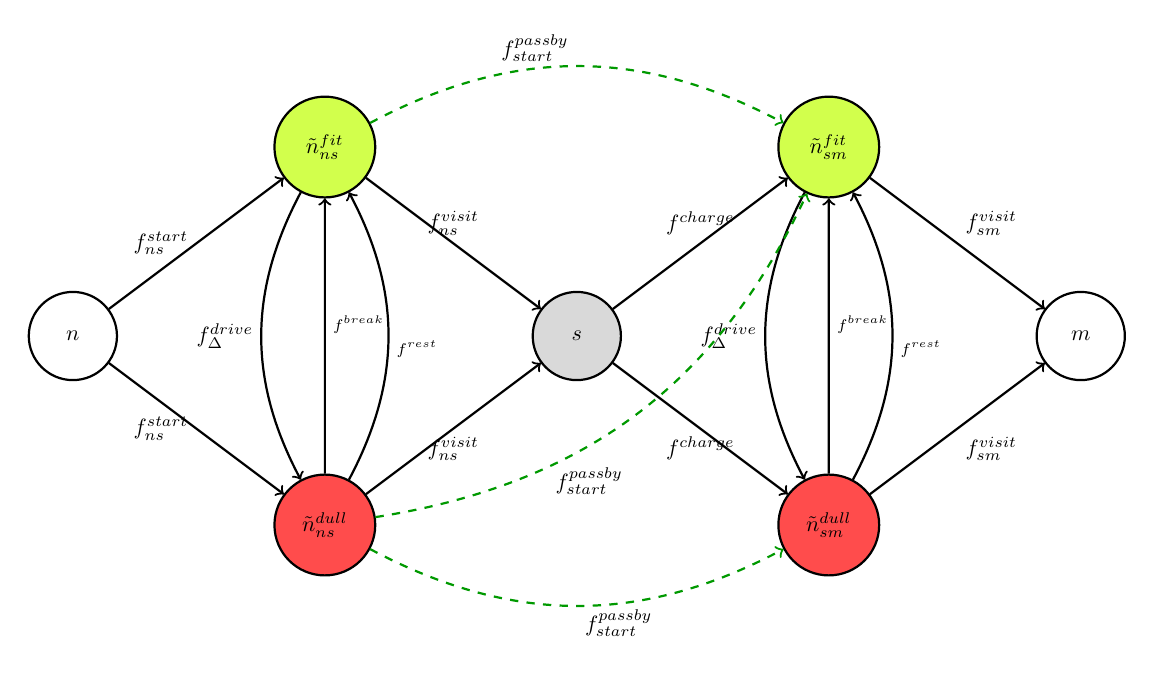
\begin{tikzpicture}[scale=0.8, transform shape, ->, thick, auto]
% Node styles
\tikzstyle{main} = [circle, draw=black, minimum size=1.4cm, inner sep=0pt]
\tikzstyle{fit}  = [circle, draw=black, fill=lime!70, minimum size=1.6cm, inner sep=0pt]
\tikzstyle{dull} = [circle, draw=black, fill=red!70, minimum size=1.6cm, inner sep=0pt]
\tikzstyle{cs}   = [circle, draw=black, fill=gray!30, minimum size=1.4cm, inner sep=0pt]

% Nodes
\node[main] (n) at (0,0) {$n$};
\node[fit]  (fitL) at (4, 3) {$\tilde{n}^{\text{fit}}_{ns}$};
\node[dull] (dullL) at (4, -3) {$\tilde{n}^{\text{dull}}_{ns}$};
\node[cs]   (cs) at (8, 0) {$s$};
\node[fit]  (fitR) at (12, 3) {$\tilde{n}^{\text{fit}}_{sm}$};
\node[dull] (dullR) at (12, -3) {$\tilde{n}^{\text{dull}}_{sm}$};
\node[main] (m) at (16,0) {$m$};

% From n to left states
\path (n) edge node[left] {$f^{\text{start}}_{ns}$} (fitL);
\path (n) edge node[left] {$f^{\text{start}}_{ns}$} (dullL);

% Transitions between fit/dull (left side)
\path[bend right=28] (fitL) edge node[left] {$f^{\text{drive}}_{\Delta}$} (dullL);
\path (dullL) edge node[right, yshift=5pt] {\scriptsize $f^{\text{break}}$} (fitL);
\path[bend right=28] (dullL) edge node[right, yshift=-6pt] {\scriptsize $f^{\text{rest}}$} (fitL);

% To s
\path (fitL) edge node[above] {$f^{\text{visit}}_{ns}$} (cs);
\path (dullL) edge node[below] {$f^{\text{visit}}_{ns}$} (cs);

% From s to right states
\path (cs) edge node[above] {$f^{\text{charge}}$} (fitR);
\path (cs) edge node[below] {$f^{\text{charge}}$} (dullR);

% Transitions between fit/dull (right side)
\path[bend right=28] (fitR) edge node[left] {$f^{\text{drive}}_{\Delta}$} (dullR);
\path (dullR) edge node[right, yshift=5pt] {\scriptsize $f^{\text{break}}$} (fitR);
\path[bend right=28] (dullR) edge node[right, yshift=-6pt] {\scriptsize $f^{\text{rest}}$} (fitR);

% From right states to m
\path (fitR) edge node[above right] {$f^{\text{visit}}_{sm}$}  (m);
\path (dullR) edge node[below right] {$f^{\text{visit}}_{sm}$} (m);

% Passing-by arcs
\path[->, dashed, thick, green!60!black, bend left=28]
  (fitL) edge node[left, yshift=8pt] {\textcolor{black}{$f^{\text{passby}}_{\text{start}}$}} (fitR);
\path[->, dashed, thick, green!60!black, bend right=28]
  (dullL) edge node[right, xshift=-40pt, yshift=-30pt] {\textcolor{black}{$f^{\text{passby}}_{\text{start}}$}} (fitR);
\path[->, dashed, thick, green!60!black, bend right=28]
  (dullL) edge node[right, yshift=-8pt] {\textcolor{black}{$f^{\text{passby}}_{\text{start}}$}} (dullR);
\end{tikzpicture}
\caption{Extended subnetwork with an intermediate charging station \(s\) and pass-by arcs under the full-recharge strategy.}
\label{fig:subnetwork_cs_full}
\end{figure}

At a charging-station node, the schedule may either initiate a charging activity or continue without charging. Charging is represented through recharge arcs originating from the charging-station node, while pass-by arcs allow the station to be traversed without stopping. Together, these arcs preserve the feasible continuation of both fit and dull driver states while introducing the operational choice of whether and where to recharge.

The pass-by arcs determine how HoS states are propagated when a charging station is traversed without stopping. The fit-to-fit pass-by arc represents a driver who reaches the charging-station location in a state that permits further driving, either because no interruption is due or because the required break or rest has already been completed. If the station is skipped, the driver therefore remains fit and can immediately begin the subleg from the charging-station location to \(m\). A fit-to-dull pass-by arc is unnecessary, since it would require another break or rest before any additional driving; the dull state is reached naturally only when a driving limit becomes binding on the subsequent subleg. The dull-to-dull pass-by arc preserves an outstanding interruption requirement: after skipping the charging station, the driver remains dull and must take a break or rest before driving toward \(m\). The dull-to-fit pass-by arc is a network connector that preserves the alternative continuations available after the charging-station node, allowing the next subleg to begin with driving and, if necessary, a break or rest to be taken later. It does not reset any HoS resource, so such a continuation is retained only when it is feasible under the current driving and working-time counters.

%------------------------------------------------%

\subsection{Full-recharge label definition}

%------------------------------------------------%

Under the full-recharge strategy, each charging stop restores the battery to full capacity. The energy state can therefore be represented by a single scalar resource \(l_{\text{reqEC}}\), which measures the energy requirement accumulated since the last recharge. Equivalently, the state of charge after any partial path is uniquely determined by \(B-l_{\text{reqEC}}\), where \(B\) denotes the battery capacity.

A full-recharge label is thus defined as
\[
\begin{aligned}
l = (&l_{\text{time}},\, l_{\text{timeToNext}},\, l_{\text{drive|R}},\\
     &l_{\text{drive|B}},\, l_{\text{elapsed|R}},\, l_{\text{elapsed|B}},\\
     &l_{\text{reqEC}})
\end{aligned}
\]
The resource \(l_{\text{reqEC}}\) is bounded by \(0 \leq l_{\text{reqEC}} \leq B\). Its design is inspired by \citet{desaulniers2016exact}, but we retain an energy-based rather than time-based representation in order to preserve flexibility across different battery capacities, charging powers, and energy-consumption rates.

%------------------------------------------------%

\subsection{Full-recharge resource extension functions}

%------------------------------------------------%

For the full-recharge strategy, charging at a station \(\mathrm{cs}\) is represented by an additional REF \(f^{\text{charge}}_{\mathrm{cs}}\). This extension resets the accumulated energy requirement \(l_{\text{reqEC}}\) to zero and increases the elapsed time by the charging duration implied by the current energy deficit and the available charging power. When charging overlaps with a legally admissible break or rest, the corresponding HoS counters are updated consistently so that synchronization between charging and regulatory interruptions is captured directly in the label propagation. In addition, pass-by arcs are modeled through \(f^{\text{passby}}_{\text{start}}\), which allows a charging station to be traversed without stopping while preserving all resource values except the remaining travel time to the next physical node. Table~\ref{tab:ref_full_recharge} summarizes the resource updates for the REFs together with the full-recharge charging and pass-by extensions.





\begin{table}[!htbp]
\caption{Resource updates for the REFs and the full-recharge charging extension.}
\label{tab:ref_full_recharge}
\centering
\small
\setlength{\tabcolsep}{2.5pt}
\renewcommand{\arraystretch}{1.15}
\resizebox{\linewidth}{!}{%
\begin{tabular}{@{}lccccccc@{}}
\toprule
\textbf{Resource} 
& \( f^{\text{start}}_{nm} \) 
& \( f^{\text{drive}}_{\Delta} \) 
& \( f^{\text{break}}_{\Delta} \) 
& \( f^{\text{rest}}_{\Delta} \) 
& \( f^{\text{visit}}_{nm} \) 
& \( f^{\text{charge}}_{\text{cs}} \) 
& \( f^{\text{passby}}_{\text{start}} \) \\
\midrule

\( l'_{\text{time}} \) 
& --- 
& \( l_{\text{time}} + \Delta \) 
& \( l_{\text{time}} + t_{\text{break}} \) 
& \( l_{\text{time}} + t_{\text{rest}} \) 
& \( l_{\text{time}} + s_m \) 
& \( \begin{cases}
l_{\text{time}} & l_{\text{elapsed|R}} = 0 \\
l_{\text{time}} + \max\left\{0, \frac{l_{\text{reqEC}}}{CP} - t_{\text{break}} \right\} & l_{\text{elapsed|B}} = 0 \\
l_{\text{time}} + \frac{l_{\text{reqEC}}}{CP} & \text{otherwise}
\end{cases} \) 
& --- \\

\( l'_{\text{timeToNext}} \) 
& \( t_{nm} \) 
& \( l_{\text{timeToNext}} - \Delta \) 
& --- 
& --- 
& --- 
& \( t_{\text{cs},m} \) 
& \( t_{\text{cs},m} \) \\

\( l'_{\text{drive|R}} \) 
& --- 
& \( l_{\text{drive|R}} + \Delta \) 
& --- 
& 0 
& --- 
& --- 
& --- \\

\( l'_{\text{drive|B}} \) 
& --- 
& \( l_{\text{drive|B}} + \Delta \) 
& 0 
& 0 
& --- 
& --- 
& --- \\

\( l'_{\text{elapsed|R}} \) 
& --- 
& \( l_{\text{elapsed|R}} + \Delta \) 
& \( l_{\text{elapsed|R}} + t_{\text{break}} \) 
& 0 
& \( l_{\text{elapsed|R}} + s_m \) 
& \( \begin{cases}
0 & l_{\text{elapsed|R}} = 0 \\
l_{\text{elapsed|R}} + \frac{l_{\text{reqEC}}}{CP} & \text{otherwise}
\end{cases} \) 
& --- \\

\( l'_{\text{elapsed|B}} \) 
& --- 
& \( l_{\text{elapsed|B}} + \Delta \) 
& 0 
& 0 
& \( l_{\text{elapsed|B}} + s_m \) 
& \( \begin{cases}
0 & l_{\text{elapsed|B}} = 0 \\
l_{\text{elapsed|B}} + \frac{l_{\text{reqEC}}}{CP} & \text{otherwise}
\end{cases} \) 
& --- \\

\( l'_{\text{reqEC}} \) 
& --- 
& \( l_{\text{reqEC}} + \Delta \cdot \alpha \) 
& --- 
& --- 
& --- 
& 0 
& --- \\

\bottomrule
\end{tabular}%
}
\end{table}

%------------------------------------------------%

\subsection{Full-recharge feasibility and dominance}

%------------------------------------------------%

Under the full-recharge strategy, energy feasibility is captured through the accumulated energy requirement since the last recharge. The scalar resource \(l_{\text{reqEC}}\) must remain within \([0,B]\) and is reset to zero by a recharge extension.

Let \(l_1\) and \(l_2\) be two labels ending at the same node. Under the full-recharge strategy, \(l_1\) dominates \(l_2\) if
\[
\begin{aligned}
&l_{\text{time}}^{(1)} \le l_{\text{time}}^{(2)},\qquad
l_{\text{timeToNext}}^{(1)} \le l_{\text{timeToNext}}^{(2)},\\
&\mathbf{l}_{\text{drive}}^{(1)} \le \mathbf{l}_{\text{drive}}^{(2)},\qquad
\mathbf{l}_{\text{elapsed}}^{(1)} \le \mathbf{l}_{\text{elapsed}}^{(2)},\\
&l_{\text{reqEC}}^{(1)} \le l_{\text{reqEC}}^{(2)}.
\end{aligned}
\]
where 
\[
\mathbf{l}_{\text{drive}}
=
\bigl(l_{\text{drive|R}},\,l_{\text{drive|B}}\bigr),
\qquad
\mathbf{l}_{\text{elapsed}}
=
\bigl(l_{\text{elapsed|R}},\,l_{\text{elapsed|B}}\bigr).
\]
If these componentwise conditions hold, \(l_2\) can be discarded because it cannot yield a better feasible completion than \(l_1\).

The scalar full-recharge dominance rule is therefore a special case of the partial-recharge dominance rule in the main text, obtained when the time and energy intervals collapse to singletons.






\newpage
\section{Summary of benchmark instances}\label{appendix:Test_Instance}

\red{We should make this openly available on say Github. Add a link}

{\scriptsize
\setlength{\tabcolsep}{3pt}
%\renewcommand{\arraystretch}{1.1}

\begin{longtable}{@{}l l r r l r r c r r r r@{}}
\caption{Key columns only. Distances in km; times in h. Abbreviations: Test = scenario/test name; Class = route class (short/med/long); K = number of clusters; N = total customers; Var = variant (Balanced/Unbalanced); Dist\_km = total route distance; Time\_h = total route time; Cust/Cl = customers per cluster; AvgCl\_km = average cluster distance; AvgIntra\_km = average intra-cluster customer distance; AvgInter\_km = average inter-cluster distance; AvgSvc\_h = average service time per customer.}
\label{tab:test_instance_config}\\

\toprule
Test & Class & K & N & Var & Dist\_km & Time\_h & Cust/Cl & AvgCl\_km & AvgIntra\_km & AvgInter\_km & AvgSvc\_h \\
\midrule
long\_cl1\_cu4 & long & 1 & 4 & - & 3929.38 & 56.1340 & [4] & 0.00 & 30.00 & 0.00 & 0.2650 \\
long\_cl2\_cu2\_Balanced & long & 2 & 2 & Balanced & 4485.46 & 64.0780 & [1,1] & 674.75 & 0.00 & 674.75 & 0.4579 \\
long\_cl2\_cu2\_Unbalanced & long & 2 & 2 & Unbalanced & 4472.53 & 63.8932 & [1,1] & 972.92 & 0.00 & 972.92 & 0.4207 \\
long\_cl2\_cu3\_Balanced & long & 2 & 3 & Balanced & 4400.36 & 62.8623 & [1,2] & 797.97 & 37.73 & 797.97 & 0.4761 \\
long\_cl2\_cu4\_Balanced & long & 2 & 4 & Balanced & 4162.88 & 59.4697 & [2,2] & 459.89 & 52.93 & 459.89 & 0.2409 \\
long\_cl2\_cu4\_Unbalanced & long & 2 & 4 & Unbalanced & 4576.22 & 65.3745 & [3,1] & 1030.26 & 103.29 & 1030.26 & 0.2304 \\
long\_cl2\_cu5\_Balanced & long & 2 & 5 & Balanced & 5119.54 & 73.1362 & [3,2] & 988.26 & 73.77 & 988.26 & 0.2437 \\
long\_cl3\_cu12\_Balanced & long & 3 & 12 & Balanced & 5097.76 & 72.8252 & [4,4,4] & 810.85 & 45.65 & 1081.13 & 0.1286 \\
long\_cl3\_cu12\_Unbalanced & long & 3 & 12 & Unbalanced & 4355.65 & 62.2236 & [1,10,1] & 647.62 & 30.00 & 863.49 & 0.1340 \\
long\_cl3\_cu14\_Balanced & long & 3 & 14 & Balanced & 5063.93 & 72.3419 & [5,5,4] & 807.74 & 30.00 & 1076.99 & 0.1190 \\
long\_cl3\_cu3\_Balanced & long & 3 & 3 & Balanced & 5016.56 & 71.6651 & [1,1,1] & 818.32 & 0.00 & 1091.09 & 0.3899 \\
long\_cl3\_cu4\_Balanced & long & 3 & 4 & Balanced & 4155.45 & 59.3636 & [2,1,1] & 680.25 & 62.77 & 907.00 & 0.2582 \\
long\_cl3\_cu4\_Unbalanced & long & 3 & 4 & Unbalanced & 5020.14 & 71.7163 & [1,2,1] & 758.57 & 50.84 & 1011.43 & 0.2508 \\
long\_cl3\_cu5\_Balanced & long & 3 & 5 & Balanced & 5518.38 & 78.8340 & [2,2,1] & 894.65 & 44.15 & 1192.87 & 0.2550 \\
med\_cl1\_cu2 & med & 1 & 2 & - & 2710.05 & 38.7150 & [2] & 0.00 & 84.81 & 0.00 & 0.4260 \\
med\_cl1\_cu4 & med & 1 & 4 & - & 2615.02 & 37.3575 & [4] & 0.00 & 30.00 & 0.00 & 0.2420 \\
med\_cl2\_cu2\_Balanced & med & 2 & 2 & Balanced & 2737.17 & 39.1024 & [1,1] & 446.85 & 0.00 & 446.85 & 0.4159 \\
med\_cl2\_cu2\_Unbalanced & med & 2 & 2 & Unbalanced & 2321.67 & 33.1667 & [1,1] & 258.77 & 0.00 & 258.77 & 0.4043 \\
med\_cl2\_cu3\_Balanced & med & 2 & 3 & Balanced & 3074.20 & 43.9171 & [1,2] & 499.00 & 43.26 & 499.00 & 0.4393 \\
med\_cl2\_cu4\_Balanced & med & 2 & 4 & Balanced & 2413.01 & 34.4716 & [2,2] & 436.35 & 42.90 & 436.35 & 0.2751 \\
med\_cl2\_cu4\_Unbalanced & med & 2 & 4 & Unbalanced & 3105.84 & 44.3691 & [2,2] & 681.02 & 73.82 & 681.02 & 0.2348 \\
med\_cl2\_cu5\_Balanced & med & 2 & 5 & Balanced & 2251.60 & 32.1658 & [3,2] & 286.03 & 47.68 & 286.03 & 0.2607 \\
med\_cl3\_cu11\_Balanced & med & 3 & 11 & Balanced & 2534.30 & 36.2043 & [4,4,3] & 332.33 & 56.27 & 443.11 & 0.1281 \\
med\_cl3\_cu13\_Balanced & med & 3 & 13 & Balanced & 2513.67 & 35.9096 & [5,4,4] & 369.80 & 30.00 & 493.07 & 0.1271 \\
med\_cl3\_cu13\_Unbalanced & med & 3 & 13 & Unbalanced & 3189.23 & 45.5604 & [2,2,9] & 437.50 & 36.03 & 583.33 & 0.1135 \\
med\_cl3\_cu3\_Balanced & med & 3 & 3 & Balanced & 3292.08 & 47.0297 & [1,1,1] & 477.29 & 0.00 & 636.38 & 0.4144 \\
med\_cl3\_cu4\_Balanced & med & 3 & 4 & Balanced & 2265.07 & 32.3581 & [2,1,1] & 360.47 & 142.64 & 480.63 & 0.2684 \\
med\_cl3\_cu4\_Unbalanced & med & 3 & 4 & Unbalanced & 2200.53 & 31.4361 & [2,1,1] & 399.06 & 132.66 & 532.08 & 0.2710 \\
med\_cl3\_cu5\_Balanced & med & 3 & 5 & Balanced & 3472.59 & 49.6084 & [2,2,1] & 559.40 & 34.92 & 745.87 & 0.2871 \\
short\_cl1\_cu2 & short & 1 & 2 & - & 1081.84 & 15.4549 & [2] & 0.00 & 39.79 & 0.00 & 0.4019 \\
% short\_cl1\_cu4 & short & 1 & 4 & - & 1265.62 & 18.0803 & [4] & 0.00 & 30.00 & 0.00 & 0.2092 \\
short\_cl2\_cu2\_Balanced & short & 2 & 2 & Balanced & 1306.92 & 18.6703 & [1,1] & 213.84 & 0.00 & 213.84 & 0.4766 \\
short\_cl2\_cu2\_Unbalanced & short & 2 & 2 & Unbalanced & 1512.53 & 21.6076 & [1,1] & 221.86 & 0.00 & 221.86 & 0.4272 \\
short\_cl2\_cu3\_Balanced & short & 2 & 3 & Balanced & 1109.01 & 15.8429 & [1,2] & 108.55 & 72.96 & 108.55 & 0.3558 \\
short\_cl2\_cu4\_Balanced & short & 2 & 4 & Balanced & 1221.36 & 17.4480 & [2,2] & 162.51 & 84.56 & 162.51 & 0.2685 \\
short\_cl2\_cu4\_Unbalanced & short & 2 & 4 & Unbalanced & 1408.63 & 20.1233 & [1,3] & 159.19 & 93.35 & 159.19 & 0.2364 \\
short\_cl2\_cu5\_Balanced & short & 2 & 5 & Balanced & 1249.49 & 17.8499 & [3,2] & 175.63 & 35.51 & 175.63 & 0.2610 \\
short\_cl3\_cu10\_Balanced & short & 3 & 10 & Balanced & 1761.42 & 25.1631 & [4,3,3] & 260.70 & 30.00 & 347.60 & 0.1333 \\
short\_cl3\_cu12\_Balanced & short & 3 & 12 & Balanced & 1941.81 & 27.7401 & [4,4,4] & 277.09 & 43.40 & 369.45 & 0.1206 \\
short\_cl3\_cu12\_Unbalanced & short & 3 & 12 & Unbalanced & 1541.88 & 22.0269 & [8,2,2] & 215.62 & 43.30 & 287.50 & 0.1268 \\
short\_cl3\_cu3\_Balanced & short & 3 & 3 & Balanced & 1450.69 & 20.7242 & [1,1,1] & 234.78 & 0.00 & 313.04 & 0.4172 \\
short\_cl3\_cu4\_Balanced & short & 3 & 4 & Balanced & 1270.79 & 18.1542 & [2,1,1] & 241.75 & 106.66 & 322.33 & 0.2682 \\
short\_cl3\_cu4\_Unbalanced & short & 3 & 4 & Unbalanced & 1324.85 & 18.9264 & [2,1,1] & 197.50 & 31.86 & 263.33 & 0.2117 \\
short\_cl3\_cu5\_Balanced & short & 3 & 5 & Balanced & 1876.99 & 26.8142 & [2,2,1] & 259.19 & 68.40 & 345.58 & 0.2621 \\
\bottomrule 
\end{longtable}
}









\newpage
%---------------------------------------------------
\section{Additional Per-Instance Comparison}
\label{appendix:diagnostics}
%---------------------------------------------------


\begin{table}[!htbp]
\centering
\caption{Near-diesel diagnostic cases in the base-case setting.}
\label{tab:near_diesel_cases}
\begin{threeparttable}
\small
\setlength{\tabcolsep}{3.5pt}
\renewcommand{\arraystretch}{1.1}
\begin{tabular}{
p{4.0cm}
S[table-format=2.2]
S[table-format=2.2]
S[table-format=1.0]
S[table-format=3.1]
S[table-format=1.0]
S[table-format=3.0]
}
\toprule
Instance & {EV (h)} & {Diesel (h)} & {CS} & {Sync. (\%)} & {Unsync.} & {Idle (min)} \\
\midrule
s\_cl2\_cu4\_U & 27.86 & 27.86 & 3 & 100.0 & 0 & 0 \\
s\_cl2\_cu3\_B   & 27.19 & 27.19 & 2 & 100.0 & 0 & 0 \\
m\_cl2\_cu2\_U   & 68.95 & 68.95 & 6 & 100.0 & 0 & 0 \\
m\_cl3\_cu4\_U   & 64.10 & 64.10 & 5 & 100.0 & 0 & 0 \\
s\_cl3\_cu10\_B  & 44.20 & 44.20 & 4 & 100.0 & 0 & 0 \\
s\_cl2\_cu4\_B   & 44.19 & 44.19 & 2 & 100.0 & 0 & 0 \\
\bottomrule
\end{tabular}
\begin{tablenotes}[flushleft]
\footnotesize
\item These are the base-case instances for which the optimized electric schedule attains the same total route time as the diesel proxy. In all six cases, every charging stop is synchronized with a mandatory break or rest.
\end{tablenotes}
\end{threeparttable}
\end{table}

{\scriptsize
\setlength{\tabcolsep}{2pt}
\renewcommand{\arraystretch}{1.0}

\begin{longtable}{@{}llrrrrrrrrrrrr@{}}
\caption{\red{Full- and partial-recharge results from the computational experiments. Times are in hours. Abbreviations: ID = short instance identifier used in the results files; Test = full instance name; F\_Time = full-recharge route time; F\_CS = number of charging stops under full recharge; F\_Sync = number of synchronized charging stops under full recharge; F\_Unsync = number of unsynchronized charging stops under full recharge; F\_Break = number of full-recharge charging stops synchronized with breaks; F\_Rest = number of full-recharge charging stops synchronized with daily rests; P\_Time = partial-recharge route time; P\_CS = number of charging stops under partial recharge; P\_Sync = number of synchronized charging stops under partial recharge; P\_Unsync = number of unsynchronized charging stops under partial recharge; P\_Break = number of partial-recharge charging stops synchronized with breaks; P\_Rest = number of partial-recharge charging stops synchronized with daily rests.}}
\label{tab:appendix_full_results}\\
\toprule
ID & Test & F\_Time & F\_CS & F\_Sync & F\_Unsync & F\_Break & F\_Rest & P\_Time & P\_CS & P\_Sync & P\_Unsync & P\_Break & P\_Rest \\
\midrule
S\_cl1\_cu2\_B & short\_cl1\_cu2 & 31.73 & 3 & 1 & 2 & 0 & 1 & 31.49 & 3 & 1 & 2 & 0 & 1 \\
S\_cl2\_cu3\_B & short\_cl2\_cu3\_Balanced & 27.27 & 1 & 1 & 0 & 0 & 1 & 27.19 & 2 & 2 & 0 & 1 & 1 \\
S\_cl2\_cu4\_B & short\_cl2\_cu4\_Balanced & 44.35 & 2 & 2 & 0 & 0 & 2 & 44.19 & 2 & 2 & 0 & 0 & 2 \\
S\_cl2\_cu4\_U & short\_cl2\_cu4\_Unbalanced & 27.94 & 1 & 1 & 0 & 0 & 1 & 27.86 & 3 & 3 & 0 & 2 & 1 \\
S\_cl2\_cu5\_B & short\_cl2\_cu5\_Balanced & 30.88 & 2 & 1 & 1 & 0 & 1 & 30.72 & 2 & 1 & 1 & 0 & 1 \\
S\_cl3\_cu10\_B & short\_cl3\_cu10\_Balanced & 44.36 & 2 & 2 & 0 & 0 & 2 & 44.20 & 4 & 4 & 0 & 2 & 2 \\
S\_cl3\_cu12\_B & short\_cl3\_cu12\_Balanced & 43.69 & 2 & 2 & 0 & 0 & 2 & 43.53 & 4 & 4 & 0 & 2 & 2 \\
S\_cl3\_cu12\_U & short\_cl3\_cu12\_Unbalanced & 30.57 & 2 & 1 & 1 & 0 & 1 & 30.16 & 2 & 2 & 0 & 1 & 1 \\
S\_cl3\_cu3\_B & short\_cl3\_cu3\_Balanced & 31.35 & 3 & 1 & 2 & 0 & 1 & 30.86 & 3 & 2 & 1 & 1 & 1 \\
S\_cl3\_cu4\_B & short\_cl3\_cu4\_Balanced & 31.18 & 2 & 1 & 1 & 0 & 1 & 31.02 & 3 & 2 & 1 & 1 & 1 \\
S\_cl3\_cu4\_U & short\_cl3\_cu4\_Unbalanced & 32.17 & 2 & 1 & 1 & 0 & 1 & 31.85 & 3 & 2 & 1 & 1 & 1 \\
S\_cl3\_cu5\_B & short\_cl3\_cu5\_Balanced & 31.48 & 2 & 1 & 1 & 0 & 1 & 31.32 & 3 & 2 & 1 & 1 & 1 \\
M\_cl1\_cu2\_B & med\_cl1\_cu2 & 68.95 & 6 & 6 & 0 & 0 & 6 & 68.95 & 6 & 6 & 0 & 0 & 6 \\
M\_cl1\_cu4\_B & med\_cl1\_cu4 & 64.26 & 5 & 4 & 1 & 0 & 4 & 64.10 & 5 & 5 & 0 & 1 & 4 \\
M\_cl2\_cu2\_B & med\_cl2\_cu2\_Balanced & 69.44 & 4 & 3 & 1 & 0 & 3 & 68.95 & 6 & 6 & 0 & 0 & 6 \\
M\_cl2\_cu2\_U & med\_cl2\_cu2\_Unbalanced & 37.11 & 2 & 2 & 0 & 0 & 2 & 36.62 & 3 & 3 & 0 & 1 & 2 \\
M\_cl2\_cu3\_B & med\_cl2\_cu3\_Balanced & 47.95 & 3 & 3 & 0 & 0 & 3 & 47.46 & 4 & 4 & 0 & 1 & 3 \\
M\_cl2\_cu4\_B & med\_cl2\_cu4\_Balanced & 64.09 & 5 & 5 & 0 & 0 & 5 & 63.60 & 7 & 7 & 0 & 2 & 5 \\
M\_cl2\_cu4\_U & med\_cl2\_cu4\_Unbalanced & 65.70 & 4 & 3 & 1 & 0 & 3 & 65.20 & 6 & 5 & 1 & 2 & 3 \\
M\_cl2\_cu5\_B & med\_cl2\_cu5\_Balanced & 37.37 & 2 & 2 & 0 & 0 & 2 & 36.88 & 3 & 3 & 0 & 1 & 2 \\
M\_cl3\_cu11\_B & med\_cl3\_cu11\_Balanced & 47.45 & 2 & 2 & 0 & 0 & 2 & 47.29 & 4 & 4 & 0 & 2 & 2 \\
M\_cl3\_cu13\_B & med\_cl3\_cu13\_Balanced & 48.39 & 2 & 2 & 0 & 0 & 2 & 48.23 & 4 & 4 & 0 & 2 & 2 \\
M\_cl3\_cu13\_U & med\_cl3\_cu13\_Unbalanced & 48.98 & 2 & 2 & 0 & 0 & 2 & 48.82 & 4 & 4 & 0 & 2 & 2 \\
M\_cl3\_cu3\_B & med\_cl3\_cu3\_Balanced & 48.66 & 4 & 3 & 1 & 0 & 3 & 47.84 & 5 & 4 & 1 & 1 & 3 \\
M\_cl3\_cu4\_B & med\_cl3\_cu4\_Balanced & 38.37 & 2 & 2 & 0 & 0 & 2 & 37.88 & 3 & 3 & 0 & 1 & 2 \\
M\_cl3\_cu4\_U & med\_cl3\_cu4\_Unbalanced & 33.00 & 2 & 2 & 0 & 0 & 2 & 32.51 & 3 & 3 & 0 & 1 & 2 \\
M\_cl3\_cu5\_B & med\_cl3\_cu5\_Balanced & 50.26 & 3 & 2 & 1 & 0 & 2 & 49.77 & 4 & 3 & 1 & 1 & 2 \\
L\_cl1\_cu2\_B & long\_cl1\_cu2 & 74.61 & 6 & 4 & 2 & 0 & 4 & 74.12 & 7 & 5 & 2 & 1 & 4 \\
L\_cl1\_cu4\_B & long\_cl1\_cu4 & 86.24 & 5 & 3 & 2 & 0 & 3 & 85.75 & 7 & 5 & 2 & 2 & 3 \\
L\_cl2\_cu2\_B & long\_cl2\_cu2\_Balanced & 75.95 & 4 & 3 & 1 & 0 & 3 & 74.65 & 7 & 6 & 1 & 2 & 4 \\
L\_cl2\_cu2\_U & long\_cl2\_cu2\_Unbalanced & 76.55 & 4 & 3 & 1 & 0 & 3 & 75.06 & 6 & 5 & 1 & 2 & 3 \\
L\_cl2\_cu3\_B & long\_cl2\_cu3\_Balanced & 76.02 & 5 & 3 & 2 & 0 & 3 & 74.53 & 7 & 5 & 2 & 2 & 3 \\
L\_cl2\_cu4\_B & long\_cl2\_cu4\_Balanced & 65.36 & 4 & 3 & 1 & 0 & 3 & 64.05 & 5 & 4 & 1 & 1 & 3 \\
L\_cl2\_cu4\_U & long\_cl2\_cu4\_Unbalanced & 79.11 & 6 & 3 & 3 & 0 & 3 & 77.81 & 8 & 5 & 3 & 2 & 3 \\
L\_cl2\_cu5\_B & long\_cl2\_cu5\_Balanced & 88.17 & 5 & 3 & 2 & 0 & 3 & 87.68 & 7 & 5 & 2 & 2 & 3 \\
L\_cl3\_cu12\_B & long\_cl3\_cu12\_Balanced & 74.79 & 4 & 4 & 0 & 0 & 4 & 74.63 & 8 & 8 & 0 & 4 & 4 \\
L\_cl3\_cu12\_U & long\_cl3\_cu12\_Unbalanced & 87.07 & 5 & 3 & 2 & 0 & 3 & 86.58 & 6 & 4 & 2 & 1 & 3 \\
L\_cl3\_cu14\_B & long\_cl3\_cu14\_Balanced & 73.33 & 4 & 4 & 0 & 0 & 4 & 73.16 & 8 & 8 & 0 & 4 & 4 \\
L\_cl3\_cu3\_B & long\_cl3\_cu3\_Balanced & 88.04 & 6 & 4 & 2 & 0 & 4 & 86.75 & 7 & 5 & 2 & 1 & 4 \\
L\_cl3\_cu4\_B & long\_cl3\_cu4\_Balanced & 76.94 & 5 & 3 & 2 & 0 & 3 & 75.45 & 7 & 5 & 2 & 2 & 3 \\
L\_cl3\_cu4\_U & long\_cl3\_cu4\_Unbalanced & 85.90 & 7 & 4 & 3 & 0 & 4 & 84.41 & 9 & 6 & 3 & 2 & 4 \\
L\_cl3\_cu5\_B & long\_cl3\_cu5\_Balanced & 98.45 & 6 & 4 & 2 & 0 & 4 & 97.96 & 8 & 6 & 2 & 2 & 4 \\
\bottomrule
\end{longtable}
}








%%%%%%%%%%%%%%%%%
\end{document}
%%%%%%%%%%%%%%%%%



